\documentclass[journal]{IEEEtran}
\usepackage[a5paper, margin=10mm]{geometry}
%\usepackage{lmodern} % Ensure lmodern is loaded for pdflatex
\usepackage{tfrupee} % Include tfrupee package

\setlength{\headheight}{1cm}
\setlength{\headsep}{0mm}

\usepackage{gvv-book}
\usepackage{gvv}
\usetikzlibrary{patterns}
\lstset{aboveskip=12pt}
\usepackage[center]{caption}
\raggedbottom
\setlength{\multicolsep}{0pt}

\hypersetup{
    colorlinks=true,
    urlcolor=black
}
\usepackage{amsfonts}
\makeindex

% The paper files reuse local label names; prefix each paper's labels and refs
% so their formula and figure links remain distinct in this combined document.
\newcommand{\paperlabelprefix}{}
\let\cbseOriginalLabel\label
\makeatletter
\renewcommand{\label}[1]{%
    \edef\cbse@labelkey{\paperlabelprefix:#1}%
    \expandafter\cbseOriginalLabel\expandafter{\cbse@labelkey}}
\AtBeginDocument{%
    \global\let\cbseOriginalRef\ref
    \renewcommand{\ref}[1]{%
        \edef\cbse@refkey{\paperlabelprefix:#1}%
        \expandafter\cbseOriginalRef\expandafter{\cbse@refkey}}}
\makeatother

\begin{document}
\bibliographystyle{IEEEtran}
\onecolumn

\title{
    \begin{center}
        CBSE 2026 Class 10 and 12 Papers\\
        \rule{0.4\columnwidth}{0.4pt}
    \end{center}
}
\author{
    \vspace{11cm}
    \begin{center}
        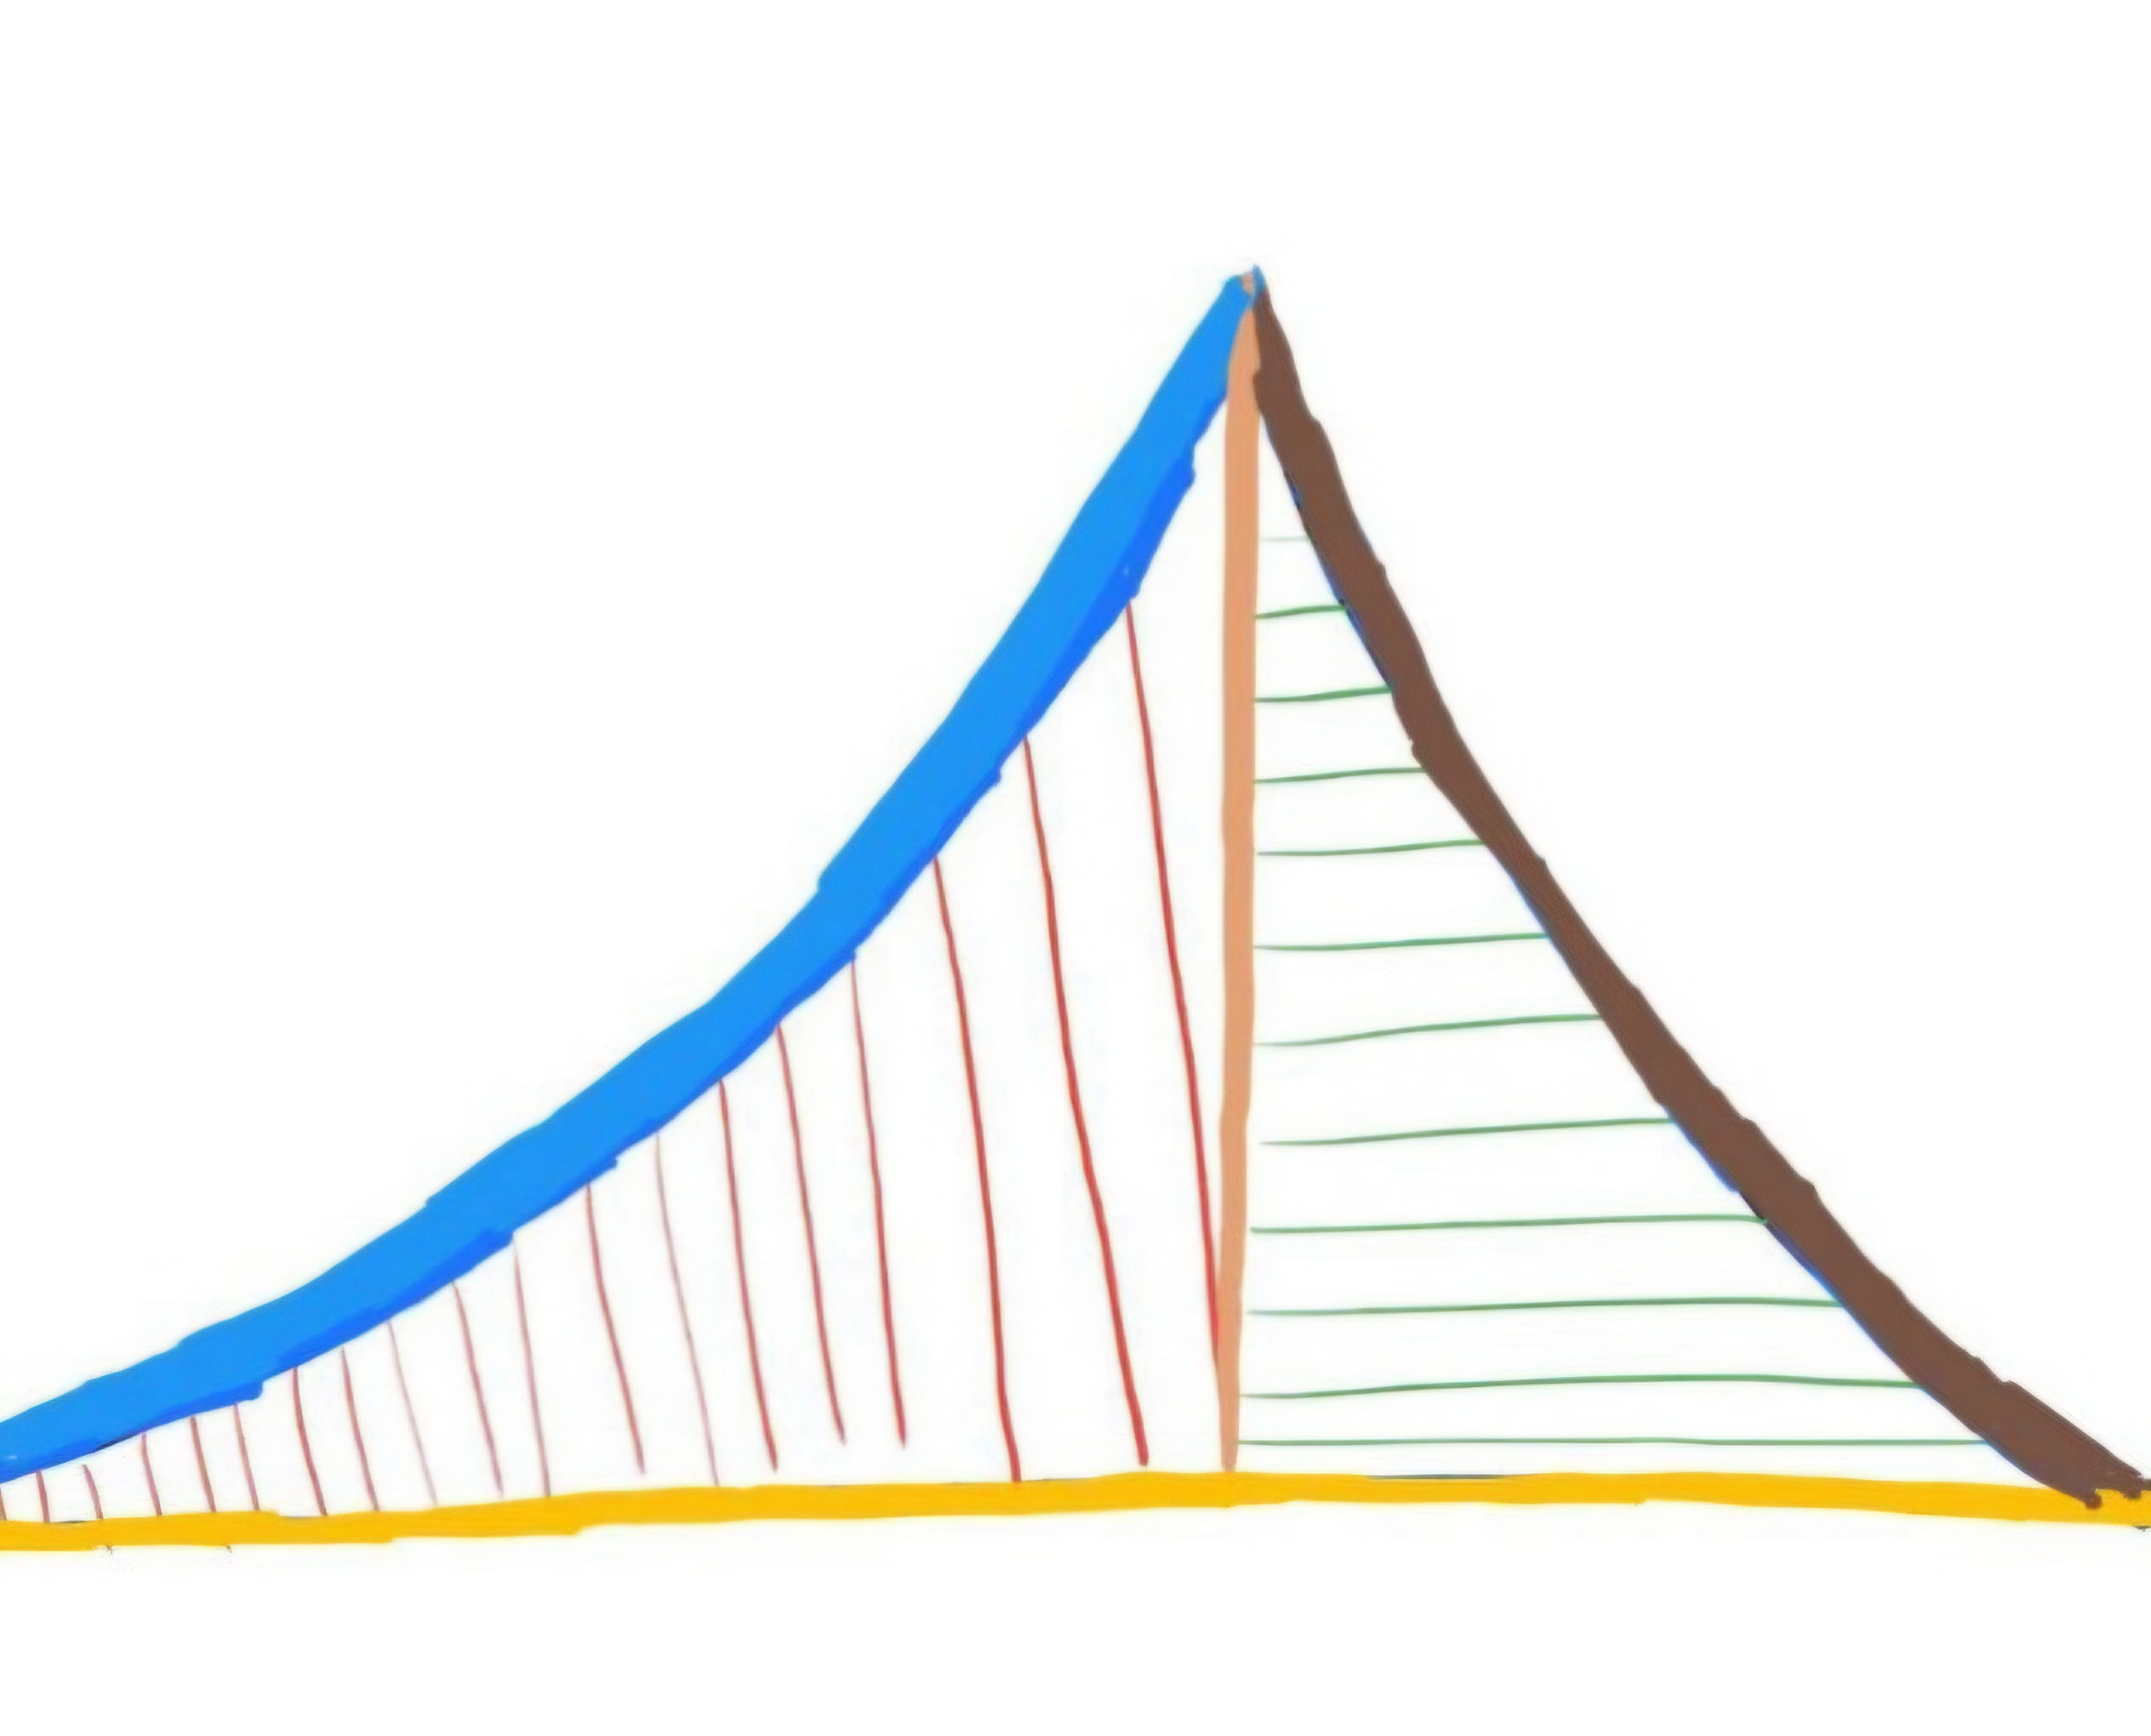
\includegraphics[width=0.2\columnwidth]{10/figs/logo.jpg}
        \\
        {\huge G. V. V. Sharma}
    \end{center}
}
\maketitle

\newpage
\section*{About this Book}

This book introduces matrices through high school coordinate geometry.
This approach makes it easier for beginners to learn Python for scientific
computing. All problems in the book are from NCERT mathematics textbooks
from Class 9--12. Exercises are from CBSE board exam papers.

The content is sufficient for industry jobs and covers nearly all matrix
prerequisites for machine learning. There is no copyright, so readers are
free to print and share.
License: https://creativecommons.org/licenses/by-sa/3.0/
\\
and
\\
https://www.gnu.org/licenses/fdl-1.3.en.html
\\
First manual appeared in January 2018
\\
First edition published on July 10, 2024
\\
In this edition, some incorrect solutions were removed. All figures
redrawn. More problems added.

\newpage
\tableofcontents
\newpage

\section{Class 10}
\subsection{Formulae}
\renewcommand{\paperlabelprefix}{10-65-3-1}
\begin{enumerate}[label=\normalfont 1.1.\arabic*.,ref=1.1.\arabic*]
\setlength{\itemsep}{0.35em}
\item \label{formula-1-1-1} \textbf{Quadratic equations.} For $ax^2+bx+c=0$,
\begin{equation*}\tag{1.1.1.1}
\Delta=b^2-4ac,\qquad x=\frac{-b\pm\sqrt{\Delta}}{2a},\qquad
\alpha+\beta=-\frac ba,\quad \alpha\beta=\frac ca.
\end{equation*}
Equal real roots occur when $\Delta=0$. For $y=ax^2+bx+c$, the vertex has $x$-coordinate $-b/(2a)$.
\item \label{formula-1-1-2} \textbf{Tangents to a circle.} A radius to the point of contact is perpendicular to the tangent. Tangents from the same external point are equal, and for radius $r$,
\begin{equation*}\tag{1.1.2.1}
PT^2=OP^2-r^2.
\end{equation*}
\item \label{formula-1-1-3} \textbf{Proportionality and similarity.} If $AB\parallel EF$ in $\triangle DEF$, then
\begin{equation*}\tag{1.1.3.1}
\frac{DA}{DE}=\frac{DB}{DF}=\frac{AB}{EF},\qquad
\frac{DA}{AE}=\frac{DB}{BF}.
\end{equation*}
For similar triangles, corresponding side ratios are equal and their area ratio is the square of that ratio.
\item \label{formula-1-1-4} \textbf{Coordinate geometry.} For $A(x_1,y_1)$ and $B(x_2,y_2)$,
\begin{equation*}\tag{1.1.4.1}
AB=\sqrt{(x_2-x_1)^2+(y_2-y_1)^2},\qquad
M=\left(\frac{x_1+x_2}{2},\frac{y_1+y_2}{2}\right).
\end{equation*}
If $AP:PB=m:n$, then $P=\left(\frac{nx_1+mx_2}{m+n},\frac{ny_1+my_2}{m+n}\right)$.
\item \label{formula-1-1-5} \textbf{Slope and parallel lines.} The slope through two points is $m=(y_2-y_1)/(x_2-x_1)$. Non-vertical parallel lines have equal slopes.
\item \label{formula-1-1-6} \textbf{Circle sectors and chords.} For a central angle $\theta$ in degrees,
\begin{equation*}\tag{1.1.6.1}
\text{arc length}=\frac{\theta}{360^\circ}2\pi r,\qquad
\text{sector area}=\frac{\theta}{360^\circ}\pi r^2.
\end{equation*}
A segment's area is the sector area minus the area of its triangle.
\item \label{formula-1-1-7} \textbf{Right-triangle trigonometry.} $\sin\theta=\frac{\text{opposite}}{\text{hypotenuse}}$, $\cos\theta=\frac{\text{adjacent}}{\text{hypotenuse}}$, and $\tan\theta=\frac{\text{opposite}}{\text{adjacent}}$.
\item \label{formula-1-1-8} \textbf{Mensuration.}
\begin{equation*}\tag{1.1.8.1}
V_{\rm cone}=\frac13\pi r^2h,\qquad
V_{\rm sphere}=\frac43\pi r^3,\qquad
S_{\rm sphere}=4\pi r^2,\qquad
S_{\rm cylinder,curved}=2\pi rh.
\end{equation*}
\item \label{formula-1-1-9} \textbf{Probability.} For equally likely outcomes, $P(E)=\frac{n(E)}{n(S)}$; $P(E^c)=1-P(E)$.
\item \label{formula-1-1-10} \textbf{HCF and LCM.} For positive integers $a,b$, $\operatorname{HCF}(a,b)\operatorname{LCM}(a,b)=ab$; the Euclidean algorithm finds the HCF by repeated division.
\item \label{formula-1-1-11} \textbf{Newton--Raphson iteration.} To approximate a root of $f(x)=0$, iterate
\begin{equation*}\tag{1.1.11.1}
x_{n+1}=x_n-\frac{f(x_n)}{f'(x_n)},\qquad f'(x_n)\ne0.
\end{equation*}
\end{enumerate}

\subsection{Solved Questions}
\renewcommand{\paperlabelprefix}{10-65-3-1}
\graphicspath{{10/}}
\begin{enumerate}[label={},font=\normalfont,leftmargin=1.15cm,labelwidth=1.0cm,labelsep=0.15cm,itemindent=0pt,listparindent=0pt,parsep=0pt,topsep=0pt]
\item[1.2.1] The roots of the quadratic equation $(x-1)^2=16$ are:

\begin{multicols}{4}
\begin{enumerate}
\setlength{\itemsep}{0pt}
    \item $5,3$
    \item $4,-4$
    \item $5,-3$
    \item $-5,3$\nobreak\hfill\mbox{(10,2026)}
\end{enumerate}
\end{multicols}



\vspace{0.6em}\par\solution

Set $f(x)=(x-1)^2-16$. The required roots satisfy $f(x)=0$, and $f'(x)=2(x-1)$. Newton--Raphson gives
\[
x_{n+1}=x_n-\frac{(x_n-1)^2-16}{2(x_n-1)},\qquad x_n\ne1.
\]
\par\noindent\hfill\mbox{\textit{(\ref{formula-1-1-11})}}\par
Starting from $x_0=0$ and $x_0=6$ gives the following iterates:
\[
\begin{array}{c|r|r}
n & x_n\;(x_0=0) & x_n\;(x_0=6)\\\hline
0 & 0.000000 & 6.000000\\
1 & -7.500000 & 5.100000\\
2 & -4.191176 & 5.001220\\
3 & -3.136665 & 5.000000\\
4 & -3.002258 & 5.000000\\
5 & -3.000001 & 5.000000\\
6 & -3.000000 & 5.000000
\end{array}
\]
Factorization independently confirms the result:
\[
(x-1)^2-16=((x-1)-4)((x-1)+4)=(x-5)(x+3)=0.
\]
Hence the exact roots are $5$ and $-3$. Substitution verifies $(5-1)^2=16$ and $(-3-1)^2=16$. These agree with the Newton--Raphson limits, while the residuals $f(x_n)$ tend to zero; therefore the iteration has found both roots. The correct answer is \textbf{c)}.

The C program prints the Newton--Raphson iterates for both starting values and returns the two roots:
\begin{lstlisting}[frame=single, basicstyle=\rmfamily, escapeinside={(*@}{@*)}]
(*@\makebox[\dimexpr\linewidth-2\fboxsep-2\fboxrule\relax][c]{codes/1.2.1.c}@*)
\end{lstlisting}
The Python program plots the two curves and marks their intersections:
\begin{lstlisting}[frame=single, basicstyle=\rmfamily, escapeinside={(*@}{@*)}]
(*@\makebox[\dimexpr\linewidth-2\fboxsep-2\fboxrule\relax][c]{codes/1.2.1.py}@*)
\end{lstlisting}
\begin{figure}[H]
    \centering
    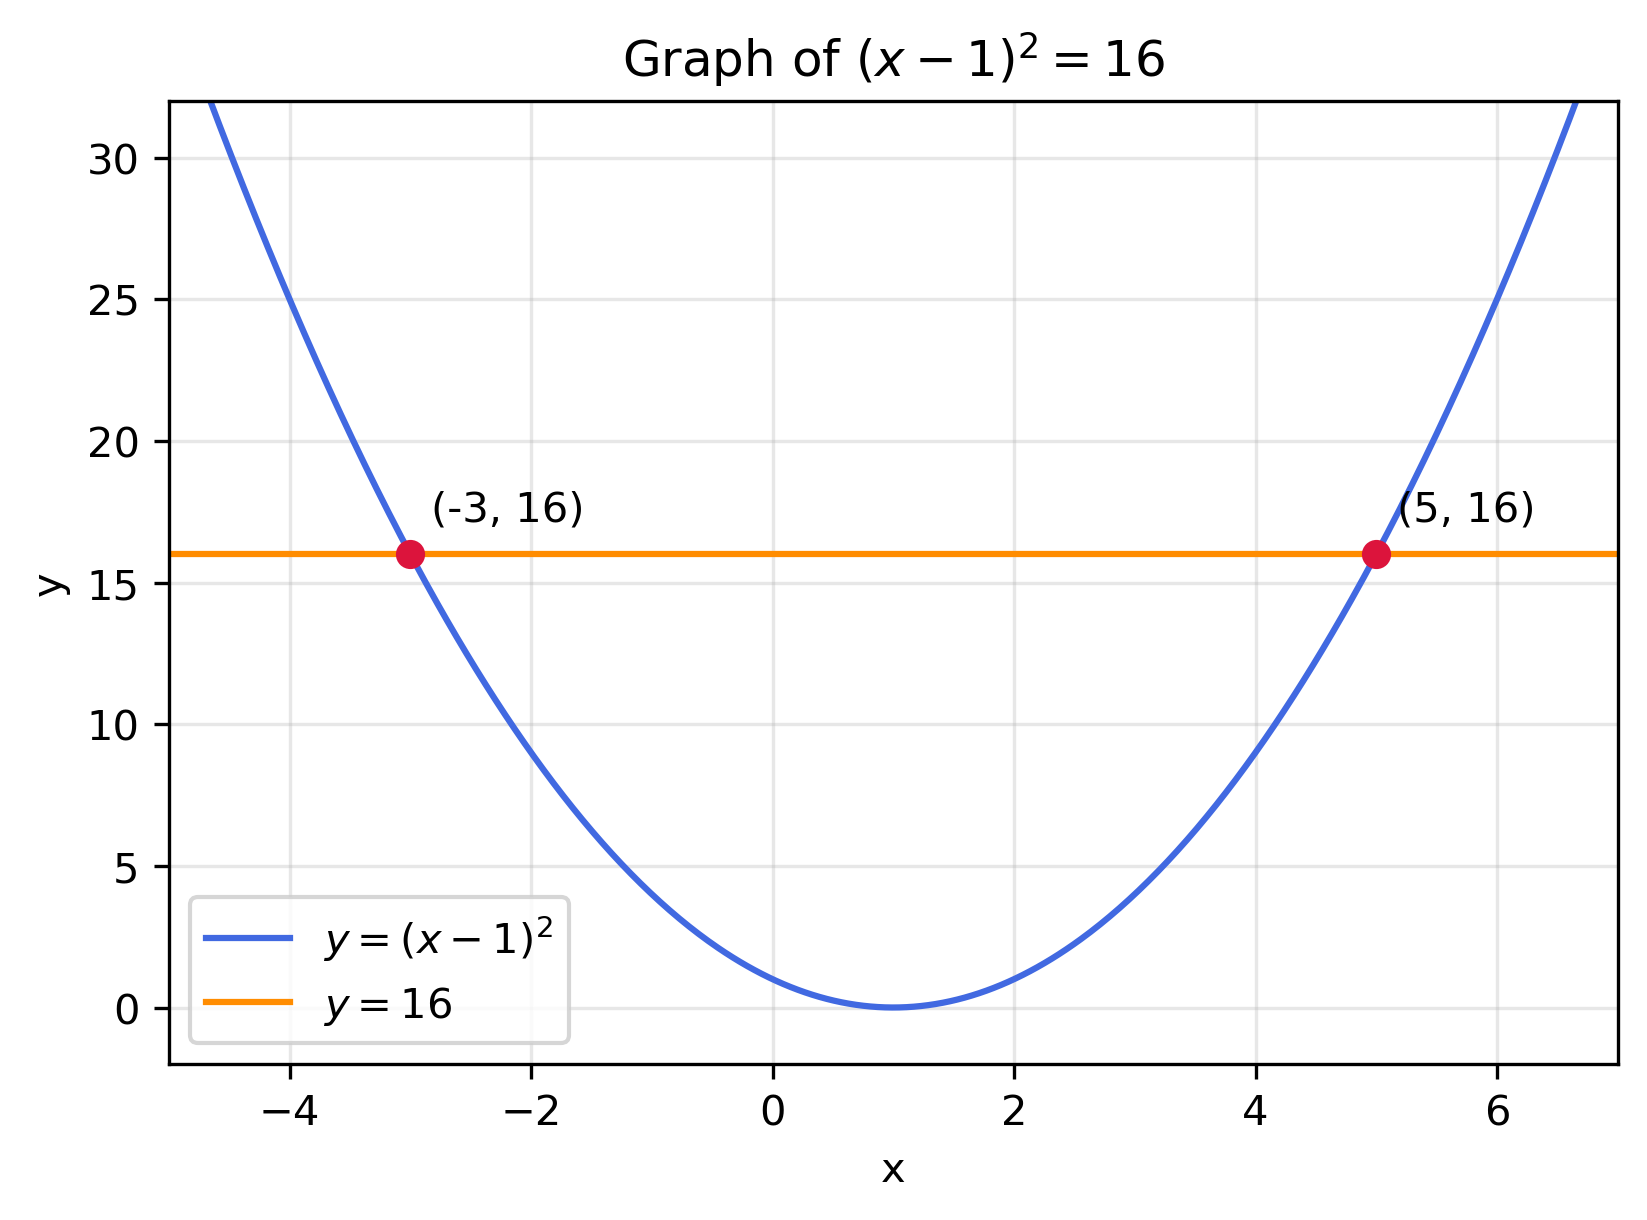
\includegraphics[width=0.48\linewidth]{figs/1.2.1.png}
    \caption{Intersections of $y=(x-1)^2$ and $y=16$, corresponding to roots $x=-3$ and $x=5$.}
\end{figure}

\item[1.2.2] In the figure, $PQ$ and $PR$ are tangents to a circle with centre $O$ and radius $3$ cm. If $\angle QPR=60^\circ$, find the length of each tangent.

\begin{multicols}{2}
\begin{enumerate}
\setlength{\itemsep}{0pt}
    \item $3\sqrt3$ cm
    \item $3$ cm
    \item $6$ cm
    \item $\sqrt3$ cm\nobreak\hfill\mbox{(10,2026)}
\end{enumerate}
\end{multicols}



\vspace{0.6em}\par\solution

The equal tangents make $OP$ bisect the $60^\circ$ angle, so $\angle QPO=30^\circ$. In right triangle $OQP$, $OP=OQ/\sin30^\circ=6$ cm. Let $\mathbf o,\mathbf p,\mathbf q,\mathbf r$ be the position vectors of the actual points, and define $\mathbf u=\mathbf p-\mathbf o$, $\mathbf v=\mathbf q-\mathbf o$, and $\mathbf w=\mathbf r-\mathbf o$. Then $\mathbf u^T\mathbf u=36$ and $\mathbf v^T\mathbf v=\mathbf w^T\mathbf w=9$. Radius-tangent perpendicularity gives
\[
\mathbf v^T(\mathbf u-\mathbf v)=0,\qquad
\mathbf w^T(\mathbf u-\mathbf w)=0,
\]
so $\mathbf u^T\mathbf v=\mathbf u^T\mathbf w=9$. Therefore
\[
\begin{aligned}
PQ^2&=(\mathbf u-\mathbf v)^T(\mathbf u-\mathbf v)=36-18+9=27,\\
PR^2&=(\mathbf u-\mathbf w)^T(\mathbf u-\mathbf w)=36-18+9=27.
\end{aligned}
\]
Hence $PQ=PR=\sqrt{27}=3\sqrt3$ cm.
\par\noindent\hfill\mbox{\textit{(\ref{formula-1-1-2})}}\par
As a consistency check, $\angle QOR=120^\circ$; hence $\mathbf v^T\mathbf w=9\cos120^\circ=-9/2$. Thus $(\mathbf q-\mathbf p)^T(\mathbf r-\mathbf p)=27/2$, and dividing by $PQ\,PR=27$ gives $\cos\angle QPR=1/2$. The given angle is satisfied, and the answer is \textbf{a)}.

The C program checks the radius, perpendicularity, equal tangent lengths and angle using vector products:
\begin{lstlisting}[frame=single, basicstyle=\rmfamily, escapeinside={(*@}{@*)}]
(*@\makebox[\dimexpr\linewidth-2\fboxsep-2\fboxrule\relax][c]{codes/1.2.2.c}@*)
\end{lstlisting}
The Python program draws the construction from the four points $O,P,Q,R$, using CoordGeo to generate the circle and line segments:
\begin{lstlisting}[frame=single, basicstyle=\rmfamily, escapeinside={(*@}{@*)}]
(*@\makebox[\dimexpr\linewidth-2\fboxsep-2\fboxrule\relax][c]{codes/1.2.2.py}@*)
\end{lstlisting}
\begin{figure}[H]
    \centering
    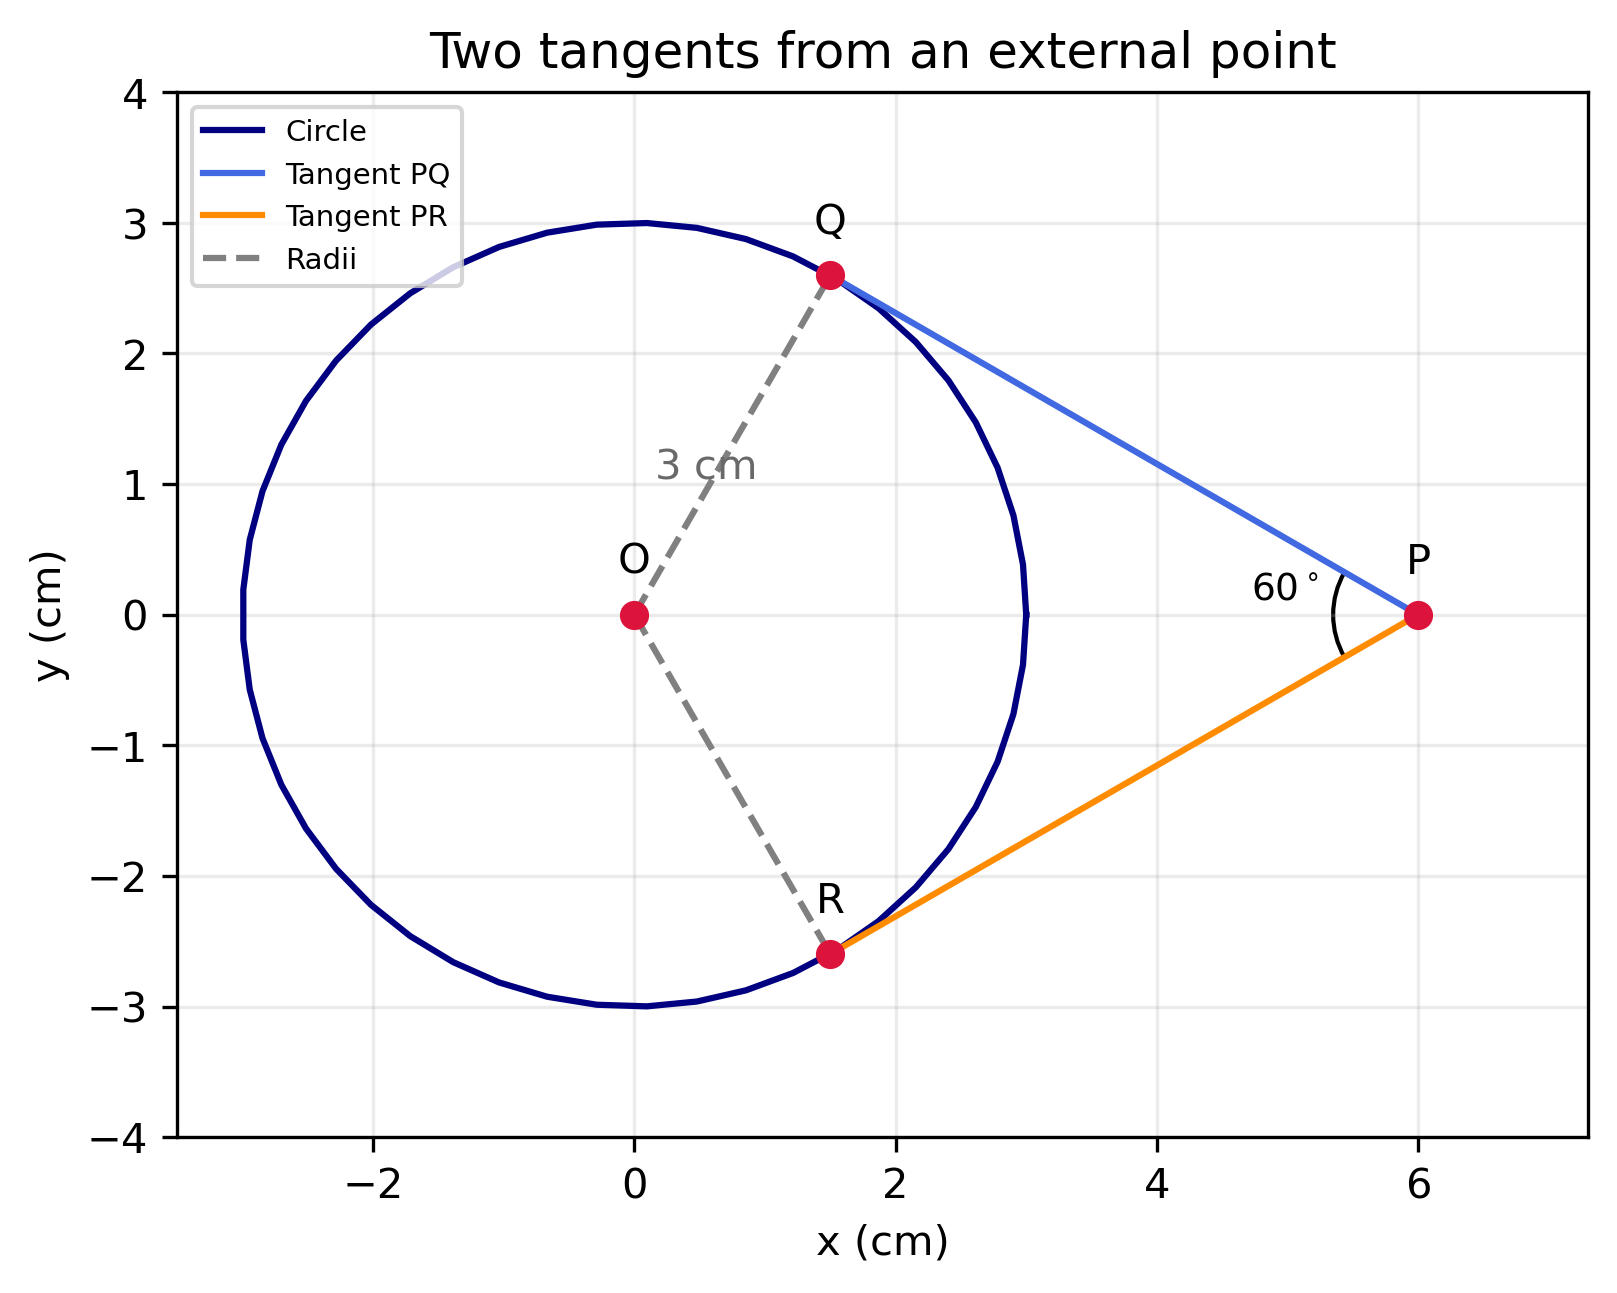
\includegraphics[width=0.47\linewidth]{figs/1.2.2.png}
    \caption{Circle with centre $O$, external point $P$, and tangent points $Q$ and $R$.}
\end{figure}

\item[1.2.3] The number $(3\times11\times13+3)$ is:

\begin{multicols}{4}
\begin{enumerate}
\setlength{\itemsep}{0pt}
    \item prime
    \item divisible by $13$
    \item composite
    \item odd\nobreak\hfill\mbox{(10,2026)}
\end{enumerate}
\end{multicols}



\vspace{0.6em}\par\solution

The following code verifies each option.
\begin{lstlisting}[frame=single, basicstyle=\rmfamily, escapeinside={(*@}{@*)}]
(*@\makebox[\dimexpr\linewidth-2\fboxsep-2\fboxrule\relax][c]{codes/1.2.3.c}@*)
\end{lstlisting}

\item[1.2.4] Two dice are rolled together. Find the probability that the sum of the numbers obtained is divisible by $6$.

\begin{multicols}{4}
\begin{enumerate}
\setlength{\itemsep}{0pt}
    \item $\frac16$
    \item $\frac{11}{36}$
    \item $\frac1{12}$
    \item $\frac14$\nobreak\hfill\mbox{(10,2026)}
\end{enumerate}
\end{multicols}



\vspace{0.6em}\par\solution


Each die can show $1$ through $6$, giving $36$ equally likely ordered pairs. For sums $2\le s\le7$, there are $s-1$ pairs, from $(1,s-1)$ through $(s-1,1)$. For sums $8\le s\le12$, the first die can show $s-6$ through $6$, giving $13-s$ pairs. Dividing these counts by $36$ gives the PMF:
\[
p_S(s)=P(S=s)=\begin{cases}
\dfrac{s-1}{36},&2\le s\le7,\\[6pt]
\dfrac{13-s}{36},&8\le s\le12,\\[6pt]
0,&\text{otherwise}.
\end{cases}
\]
The sum is divisible by $6$ only for $S=6$ and $S=12$. Therefore, using the PMF,
\[
P(S\text{ is divisible by }6)=P(S=6)+P(S=12)=\frac5{36}+\frac1{36}=\boxed{\frac16},
\]
option \textbf{a)}. The Python code uses NumPy's random number generator to simulate dice rolls and plots the simulated PMF alongside the exact PMF.
\par\noindent\hfill\mbox{\textit{(\ref{formula-1-1-9})}}\par\begin{lstlisting}[frame=single, basicstyle=\rmfamily, escapeinside={(*@}{@*)}]
(*@\makebox[\dimexpr\linewidth-2\fboxsep-2\fboxrule\relax][c]{codes/1.2.4.py}@*)
\end{lstlisting}
\begin{figure}[H]
    \centering
    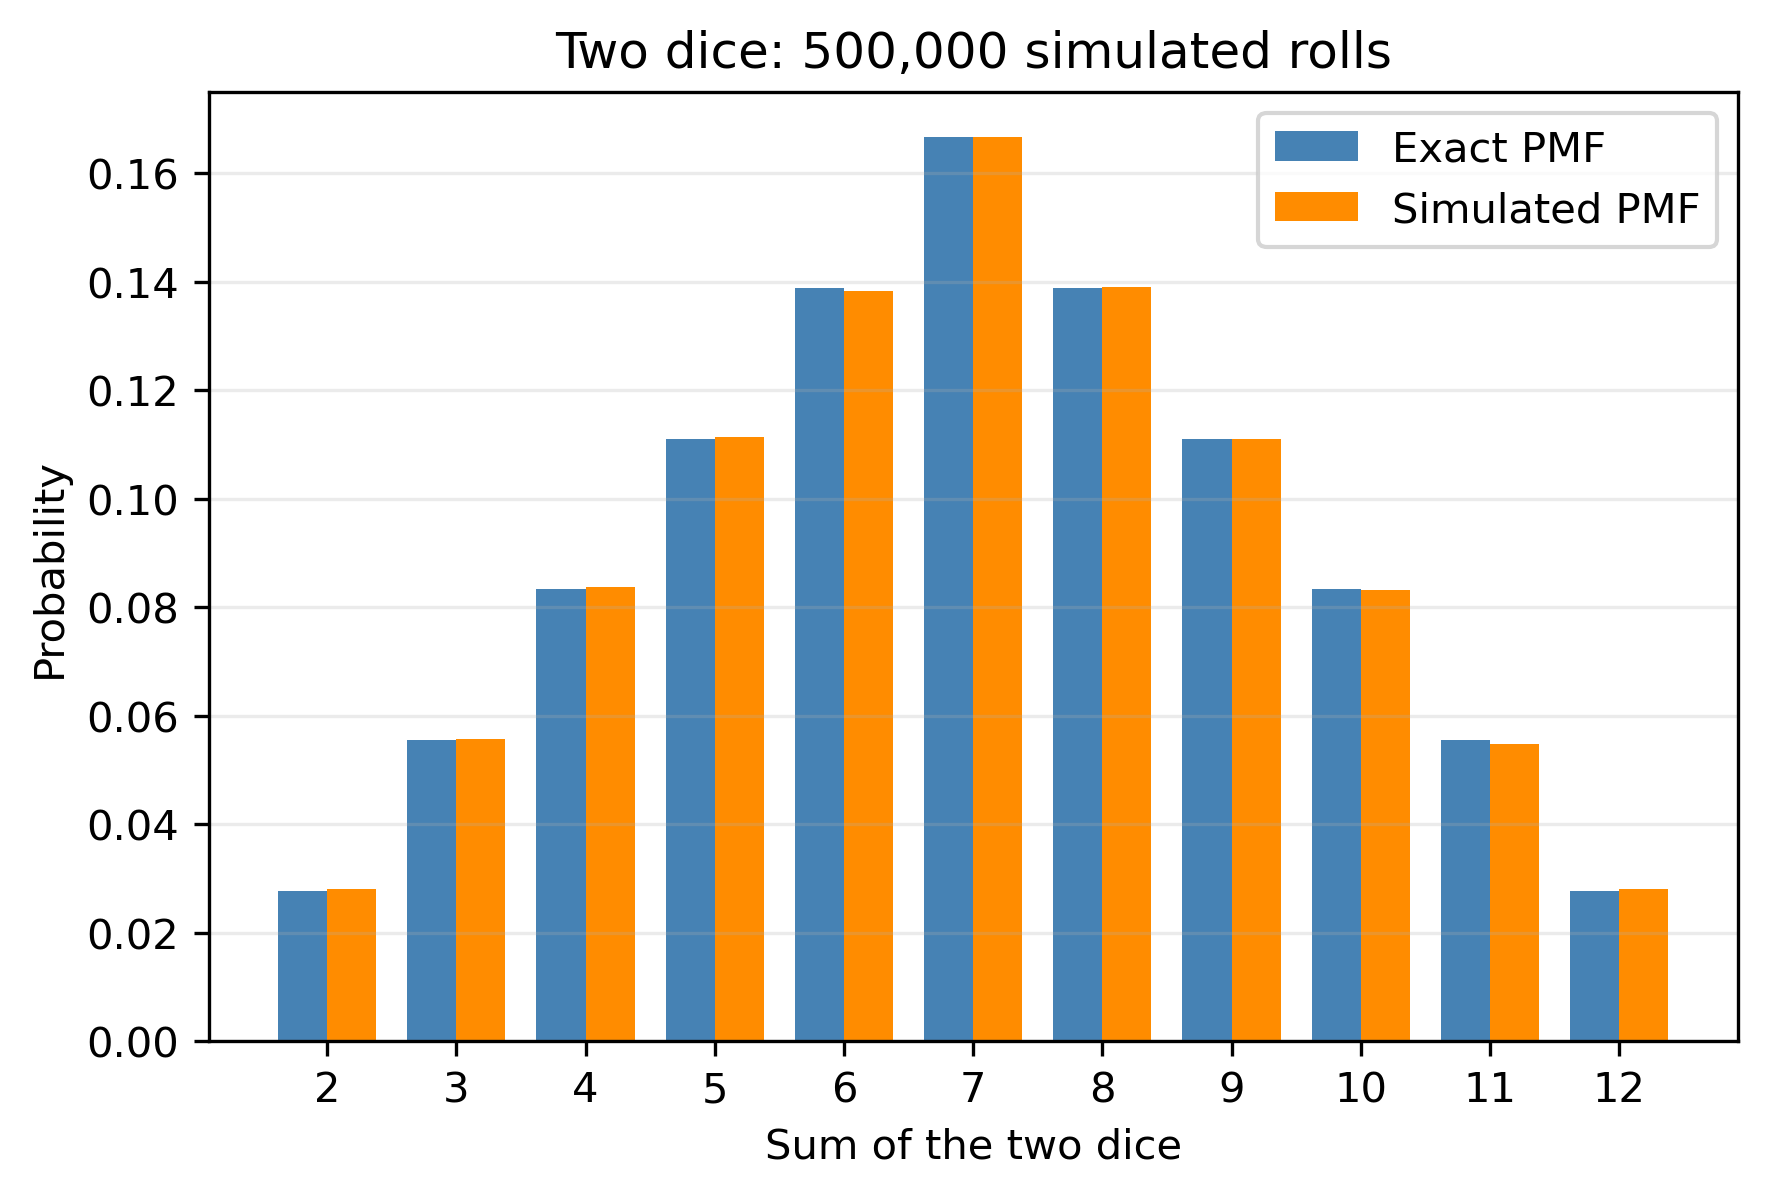
\includegraphics[width=0.50\linewidth]{figs/1.2.4.png}
    \caption{Simulated and exact probability distributions for the sum of two dice.}
\end{figure}

\item[1.2.5] The equation of another line parallel to $2x-6y=7$ is:

\begin{multicols}{2}
\begin{enumerate}
\setlength{\itemsep}{0pt}
    \item $y=3x-7$
    \item $2x=9-6y$
    \item $x-3y=7$
    \item $x=\frac72-3y$\nobreak\hfill\mbox{(10,2026)}
\end{enumerate}
\end{multicols}



\vspace{0.6em}\par\solution


The given line has slope $\frac13$. Only option c), $y=\frac13x-\frac73$, has the same slope and a different intercept. Hence the answer is \textbf{c)}. The code plots the given line and all four options.
\par\noindent\hfill\mbox{\textit{(\ref{formula-1-1-5})}}\par\begin{lstlisting}[frame=single, basicstyle=\rmfamily, escapeinside={(*@}{@*)}]
(*@\makebox[\dimexpr\linewidth-2\fboxsep-2\fboxrule\relax][c]{codes/1.2.5.py}@*)
\end{lstlisting}
\begin{figure}[H]
    \centering
    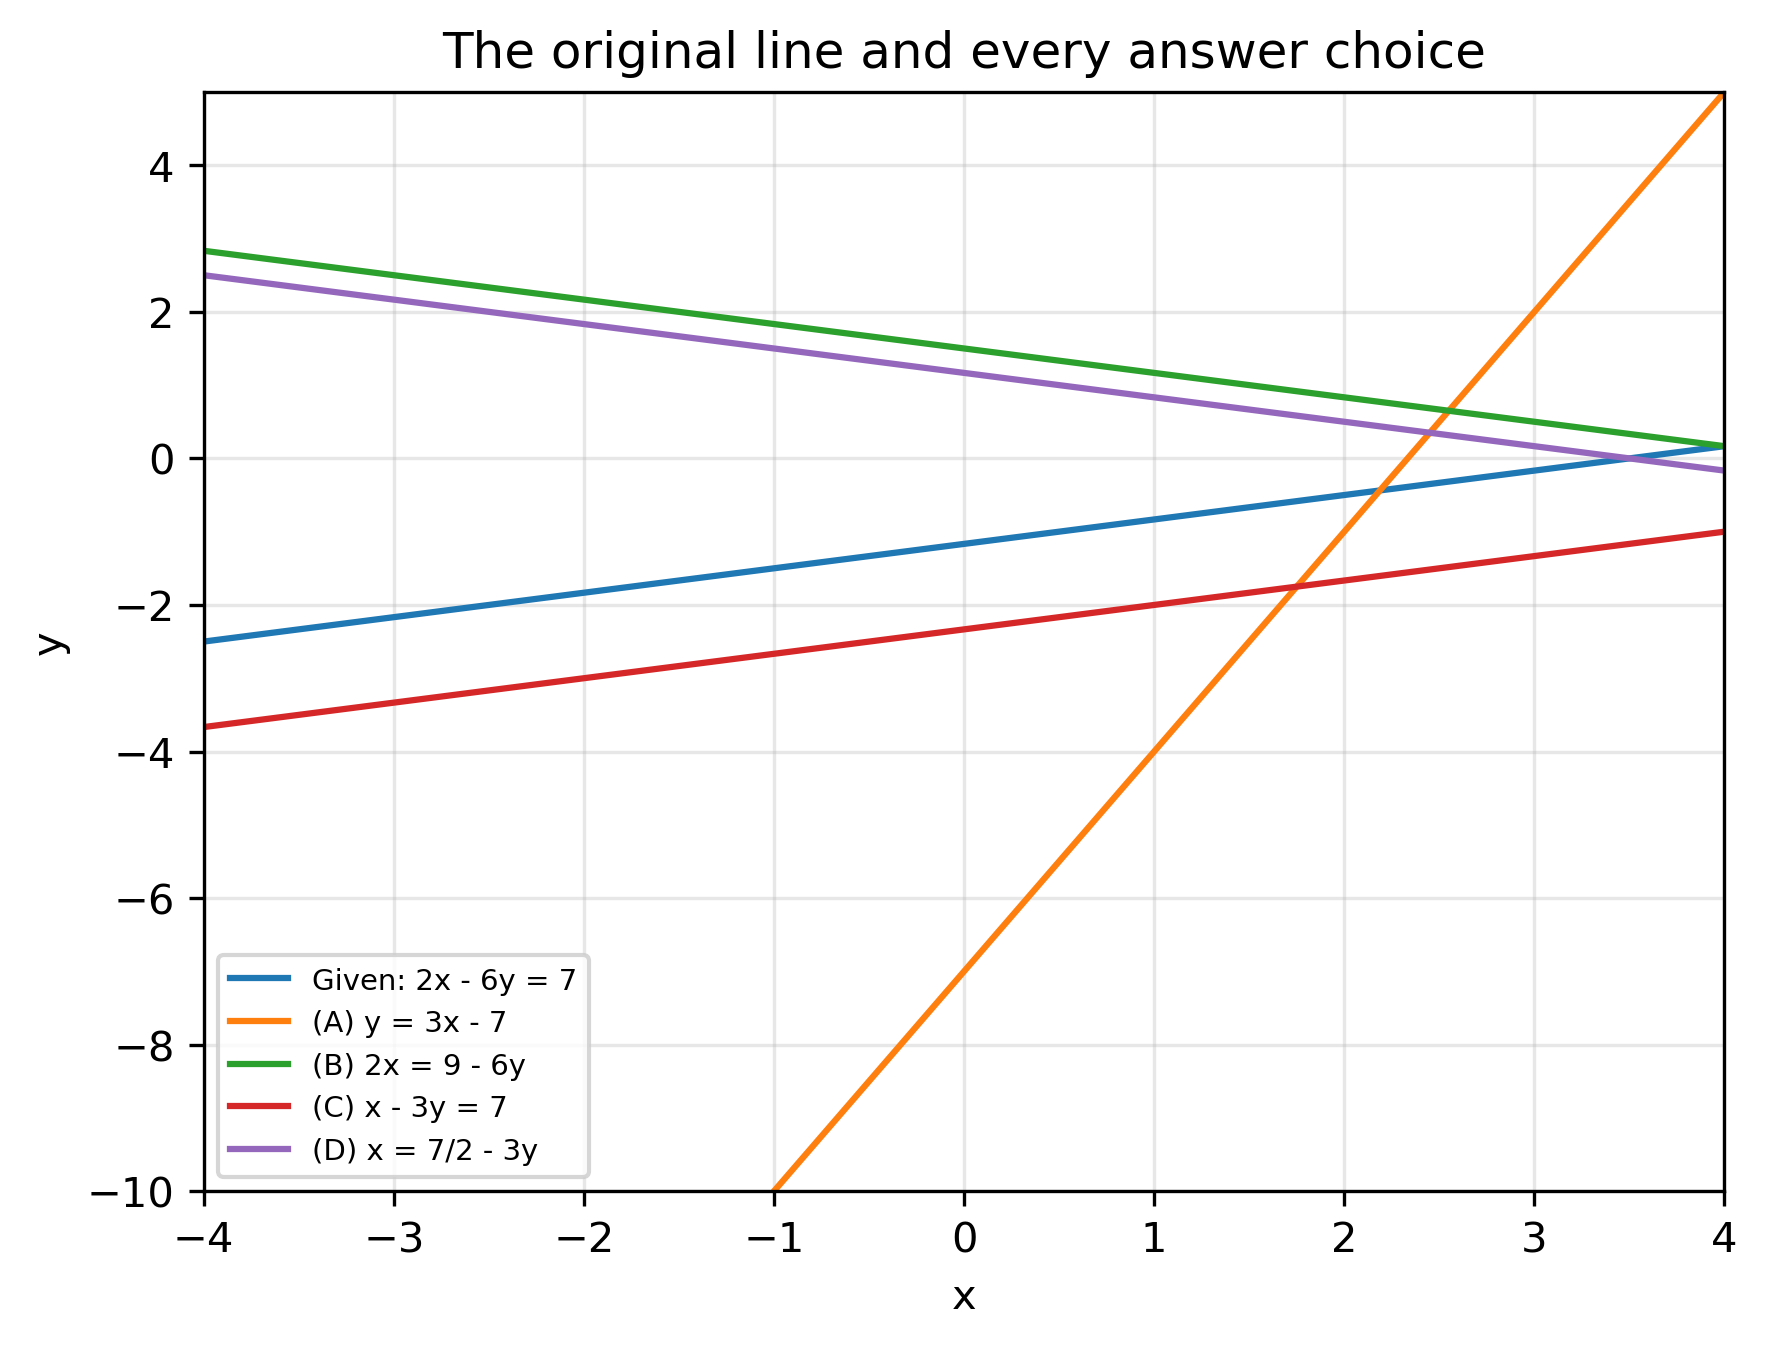
\includegraphics[width=0.52\linewidth]{figs/1.2.5.png}
    \caption{The given line and the four candidate lines.}
\end{figure}

\item[1.2.6] If the roots of $\sqrt3x^2-kx+2\sqrt3=0$ are real and equal, find the value(s) of $k$.

\begin{multicols}{4}
\begin{enumerate}
\setlength{\itemsep}{0pt}
    \item $\pm\sqrt{24}$
    \item $0$
    \item $4$
    \item $-5$\nobreak\hfill\mbox{(10,2026)}
\end{enumerate}
\end{multicols}



\vspace{0.6em}\par\solution

For $\sqrt3x^2-kx+2\sqrt3=0$, the discriminant is $D(k)=k^2-24$. Equal real roots require $D(k)=0$. Apply Newton--Raphson to $g(k)=k^2-24$, whose derivative is $g'(k)=2k$:
\[
k_{n+1}=k_n-\frac{k_n^2-24}{2k_n},\qquad k_n\ne0.
\]
\par\noindent\hfill\mbox{\textit{(\ref{formula-1-1-1}, \ref{formula-1-1-11})}}\par
Starting from $k_0=-4$ and $k_0=4$ gives
\[
\begin{array}{c|r|r}
n&k_n\;(k_0=-4)&k_n\;(k_0=4)\\\hline
0&-4.000000&4.000000\\
1&-5.000000&5.000000\\
2&-4.900000&4.900000\\
3&-4.898980&4.898980\\
4&-4.898979&4.898979
\end{array}
\]
Factorization confirms the limits: $k^2-24=(k-2\sqrt6)(k+2\sqrt6)$, so $k=\pm2\sqrt6=\pm\sqrt{24}$. Substituting these values into the original quadratic gives $\sqrt3(x-\sqrt2)^2=0$ for $k=2\sqrt6$ and $\sqrt3(x+\sqrt2)^2=0$ for $k=-2\sqrt6$. Thus each value gives a repeated real root, verifying the iteration. The correct answer is \textbf{a)}.

The C program applies Newton--Raphson from both starting values and verifies the repeated roots:
\begin{lstlisting}[frame=single, basicstyle=\rmfamily, escapeinside={(*@}{@*)}]
(*@\makebox[\dimexpr\linewidth-2\fboxsep-2\fboxrule\relax][c]{codes/1.2.6.c}@*)
\end{lstlisting}
The Python program only plots the two resulting parabolas:
\begin{lstlisting}[frame=single, basicstyle=\rmfamily, escapeinside={(*@}{@*)}]
(*@\makebox[\dimexpr\linewidth-2\fboxsep-2\fboxrule\relax][c]{codes/1.2.6.py}@*)
\end{lstlisting}
\begin{figure}[H]
    \centering
    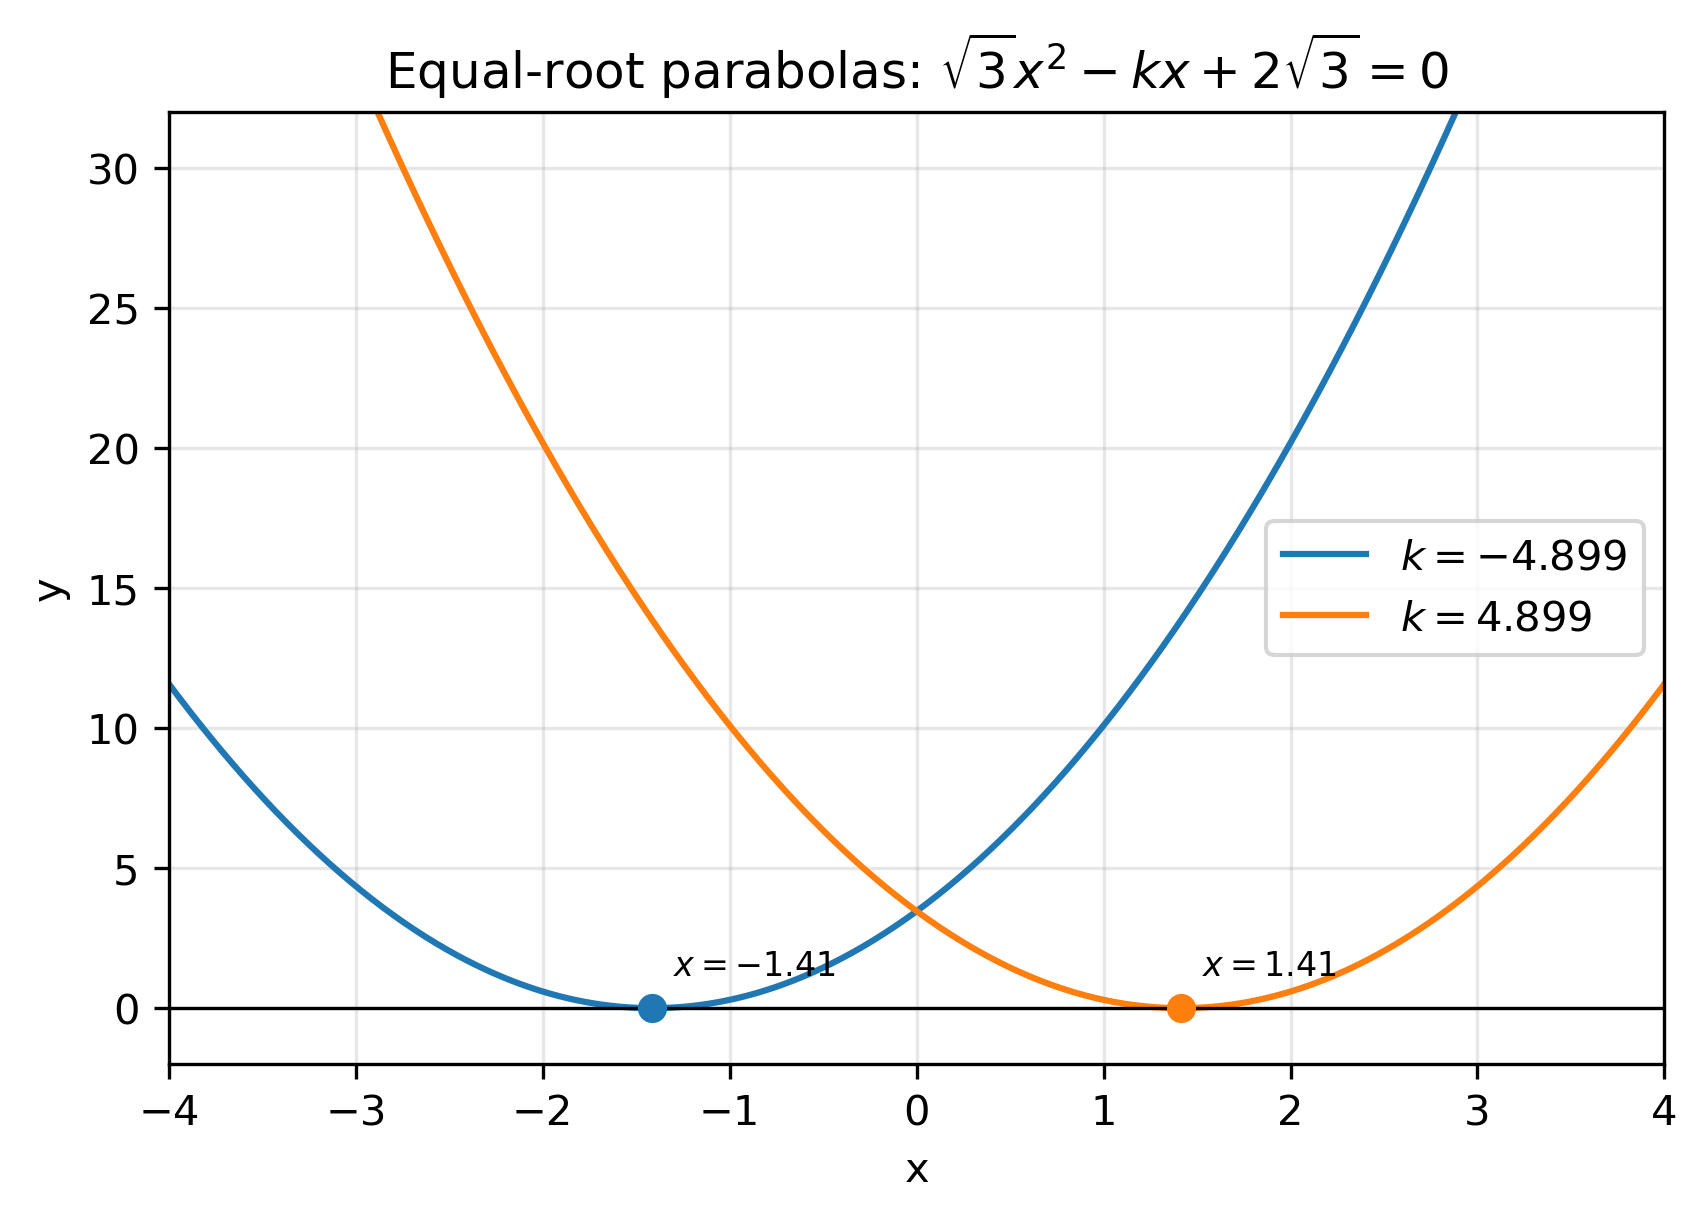
\includegraphics[width=0.52\linewidth]{figs/1.2.6.png}
    \caption{The two parabolas touching the $x$-axis at their repeated roots.}
\end{figure}

\item[1.2.7] A tangent $PT$ is drawn to a circle with centre $O$ and radius $r$. If $\angle POT=45^\circ$, find $OP$.

\begin{multicols}{4}
\begin{enumerate}
\setlength{\itemsep}{0pt}
    \item $r\sqrt2$
    \item $\sqrt{2r}$
    \item $2r$
    \item $r^2$\nobreak\hfill\mbox{(10,2026)}
\end{enumerate}
\end{multicols}



\vspace{0.6em}\par\solution


Since $OT\perp PT$, $\triangle OTP$ is right-angled at $T$. With $\angle POT=45^\circ$, it is a $45^\circ$-$45^\circ$-$90^\circ$ triangle, so $OP=r\sqrt2$. The answer is \textbf{a)}. The code draws the circle, tangent, and radius and calculates $OP$.
\par\noindent\hfill\mbox{\textit{(\ref{formula-1-1-2}, \ref{formula-1-1-7})}}\par\begin{lstlisting}[frame=single, basicstyle=\rmfamily, escapeinside={(*@}{@*)}]
(*@\makebox[\dimexpr\linewidth-2\fboxsep-2\fboxrule\relax][c]{codes/1.2.7.py}@*)
\end{lstlisting}
\begin{figure}[H]
    \centering
    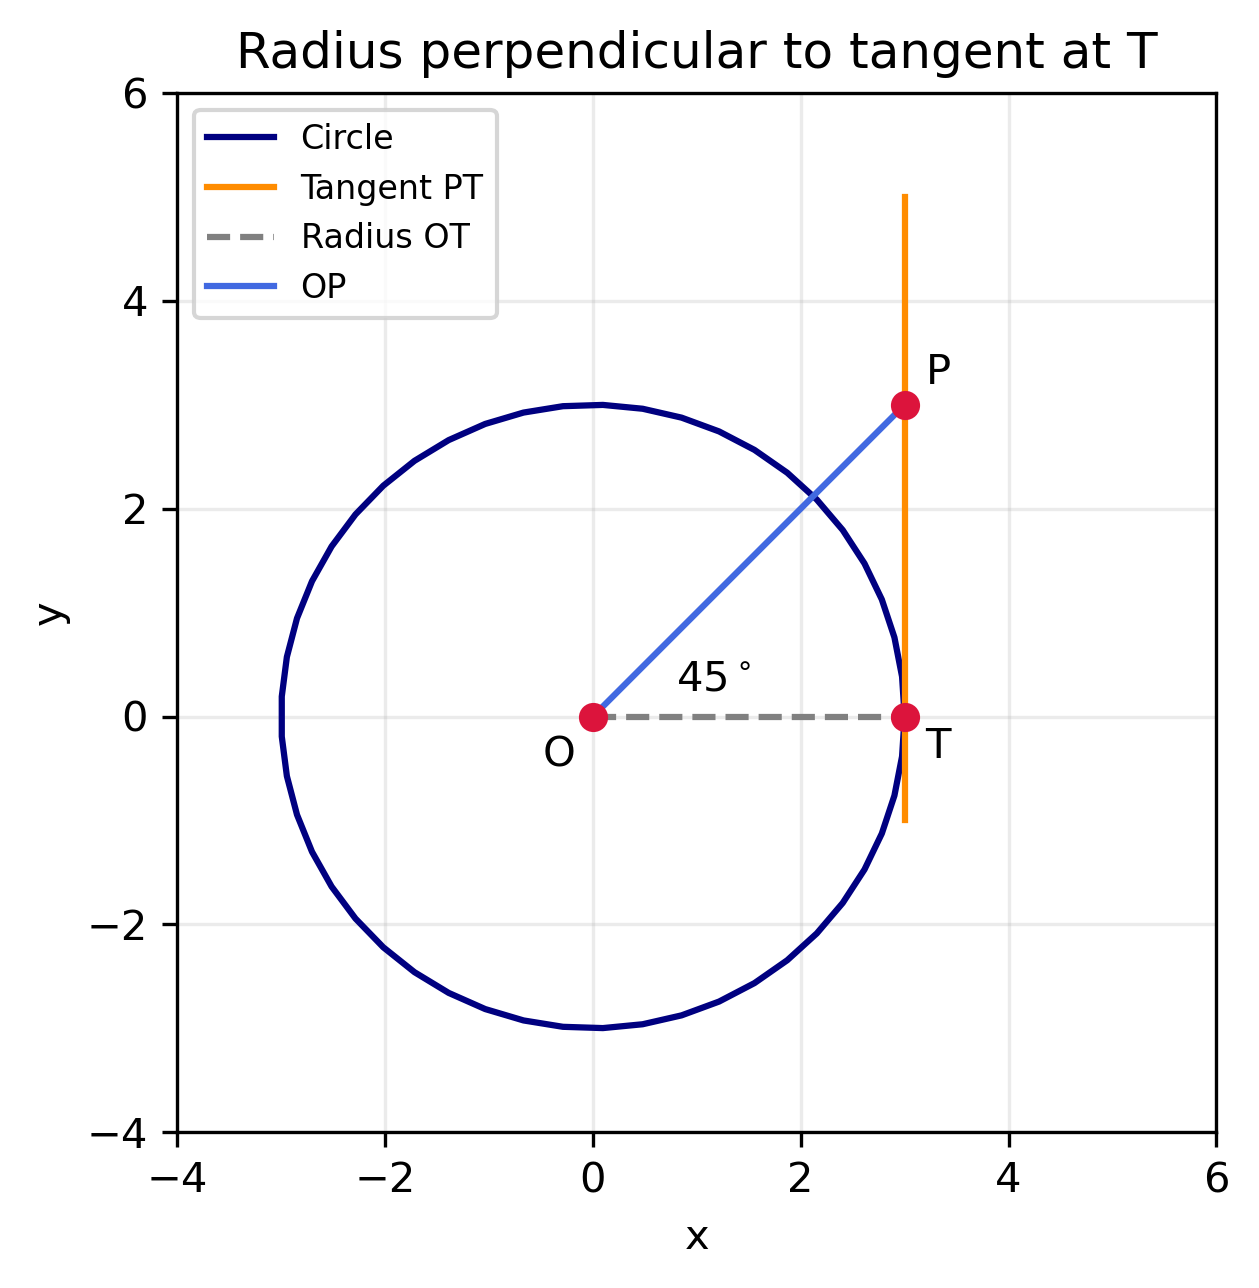
\includegraphics[width=0.48\linewidth]{figs/1.2.7.png}
    \caption{Tangent $PT$ perpendicular to radius $OT$.}
\end{figure}

\item[1.2.8] The sum and product of the zeroes of a quadratic polynomial $p(x)$ are $-\frac13$ and $2$ respectively. The polynomial $p(x)$ is:

\begin{multicols}{2}
\begin{enumerate}
\setlength{\itemsep}{0pt}
    \item $3x^2-x+6$
    \item $x^2+\frac13x-2$
    \item $3x^2-x+2$
    \item $-3x^2-x-6$\nobreak\hfill\mbox{(10,2026)}
\end{enumerate}
\end{multicols}



\vspace{0.6em}\par\solution

For $ax^2+bx+c$, the sum and product of zeroes are $-b/a$ and $c/a$. Option d) gives $-1/3$ and $2$, so it is correct. Its graph has no real zeroes, consistent with its negative discriminant.
\par\noindent\hfill\mbox{\textit{(\ref{formula-1-1-1})}}\par
The C program finds both roots by Newton--Raphson and checks their sum and product:
\begin{lstlisting}[frame=single, basicstyle=\rmfamily, escapeinside={(*@}{@*)}]
(*@\makebox[\dimexpr\linewidth-2\fboxsep-2\fboxrule\relax][c]{codes/1.2.8.c}@*)
\end{lstlisting}
The Python program only plots the selected polynomial:
\begin{lstlisting}[frame=single, basicstyle=\rmfamily, escapeinside={(*@}{@*)}]
(*@\makebox[\dimexpr\linewidth-2\fboxsep-2\fboxrule\relax][c]{codes/1.2.8.py}@*)
\end{lstlisting}
\begin{figure}[H]
    \centering
    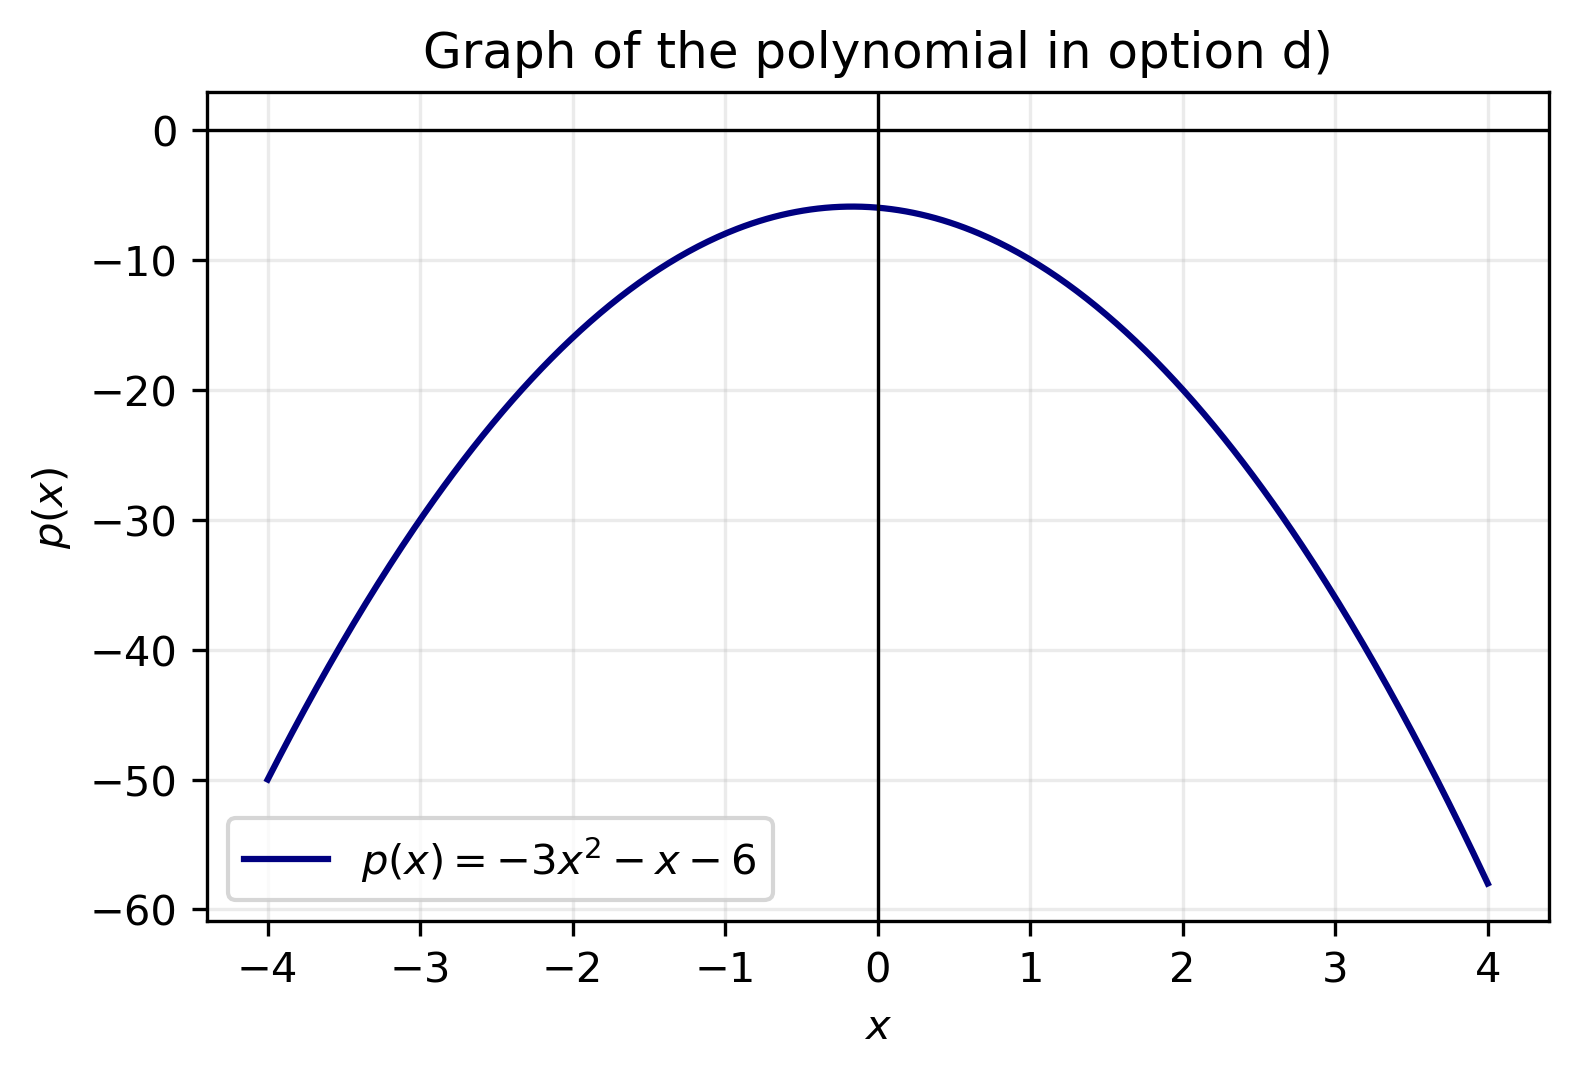
\includegraphics[width=0.51\linewidth]{figs/1.2.8.png}
    \caption{Graph of option d), which has no real zeroes.}
\end{figure}

\item[1.2.9] Find the length of a plank that can measure $4$ m $20$ cm and $5$ m $4$ cm exactly, in the least time.\nobreak\hfill\mbox{(10,2026)}



\vspace{0.6em}\par\solution


Convert the lengths to $420$ cm and $504$ cm. Euclid's algorithm uses the recurrence
\[
(a_{n+1},b_{n+1})=(b_n,\,a_n-q_nb_n),\qquad q_n=\left\lfloor\frac{a_n}{b_n}\right\rfloor,
\]
until $b_n=0$. The remainder sequence is $504,420,84,0$, so the greatest plank length is $\boxed{84\text{ cm}}$. The C program prints the recurrence steps.
\par\noindent\hfill\mbox{\textit{(\ref{formula-1-1-10})}}\par\begin{lstlisting}[frame=single, basicstyle=\rmfamily, escapeinside={(*@}{@*)}]
(*@\makebox[\dimexpr\linewidth-2\fboxsep-2\fboxrule\relax][c]{codes/1.2.9.c}@*)
\end{lstlisting}

\item[1.2.10] Diagonals $AC$ and $BD$ of square $ABCD$ intersect at $P$. Coordinates of $B$ and $D$ are $(9,-2)$ and $(1,6)$ respectively. (i) Find coordinates of $P$. (ii) Find the side length of the square.\nobreak\hfill\mbox{(10,2026)}



\vspace{0.6em}\par\solution


The diagonals bisect each other, so $P$ is the midpoint of $BD$: $P=(5,2)$. The diagonal length is $BD=\sqrt{8^2+(-8)^2}=8\sqrt2$, hence the square's side is $BD/\sqrt2=8$. The code plots the square and its diagonals.
\par\noindent\hfill\mbox{\textit{(\ref{formula-1-1-4})}}\par\begin{lstlisting}[frame=single, basicstyle=\rmfamily, escapeinside={(*@}{@*)}]
(*@\makebox[\dimexpr\linewidth-2\fboxsep-2\fboxrule\relax][c]{codes/1.2.10.py}@*)
\end{lstlisting}
\begin{figure}[H]
    \centering
    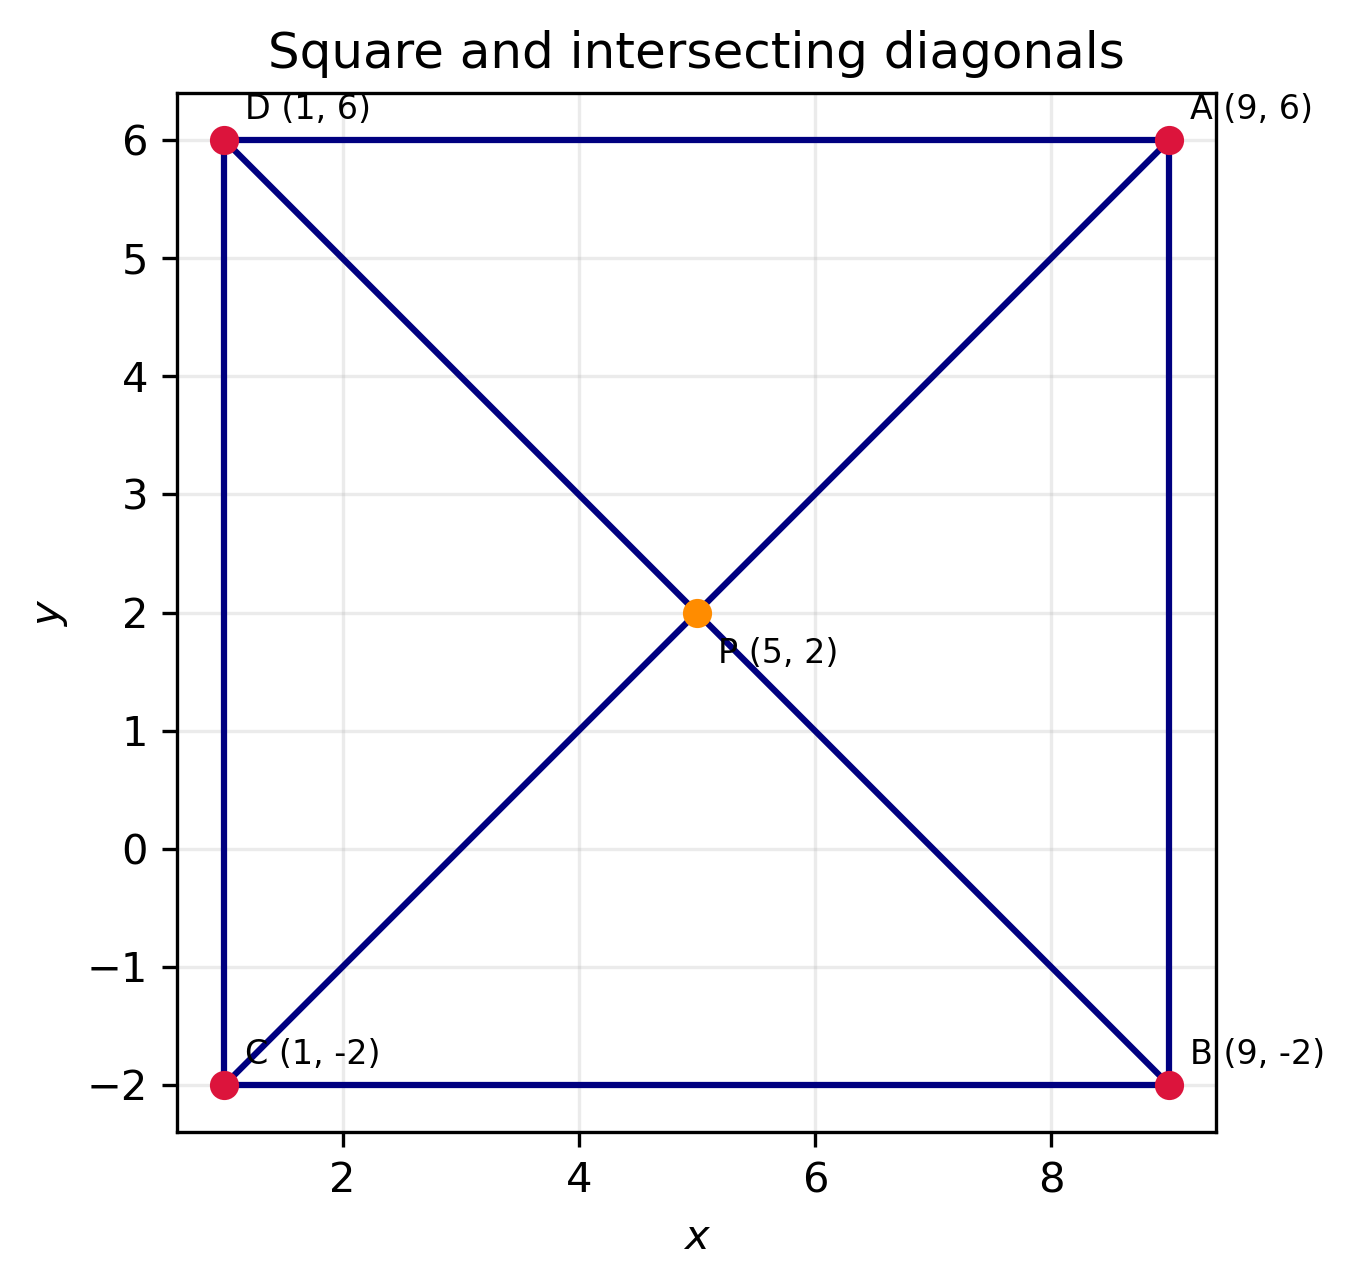
\includegraphics[width=0.49\linewidth]{figs/1.2.10.png}
    \caption{Square $ABCD$ and diagonals meeting at $P$.}
\end{figure}

\item[1.2.11] A chord $AB$ of a circle of radius $7$ cm subtends an angle of $120^\circ$ at the centre. Find (i) the perimeter of major sector $OACB$, and (ii) the area of the shaded segment if $[\triangle OAB]=21.2$ cm$^2$.\nobreak\hfill\mbox{(10,2026)}



\vspace{0.6em}\par\solution


The major arc is $240^\circ$, so the major-sector perimeter is $14+\frac{240}{360}(14\pi)=14+\frac{28\pi}{3}\approx43.32$ cm. The shaded minor segment has area $\frac{120}{360}\pi(7)^2-21.2=\frac{49\pi}{3}-21.2\approx30.11$ cm$^2$. The code draws and shades the segment and calculates both values.
\par\noindent\hfill\mbox{\textit{(\ref{formula-1-1-6})}}\par\begin{lstlisting}[frame=single, basicstyle=\rmfamily, escapeinside={(*@}{@*)}]
(*@\makebox[\dimexpr\linewidth-2\fboxsep-2\fboxrule\relax][c]{codes/1.2.11.py}@*)
\end{lstlisting}
\begin{figure}[H]
    \centering
    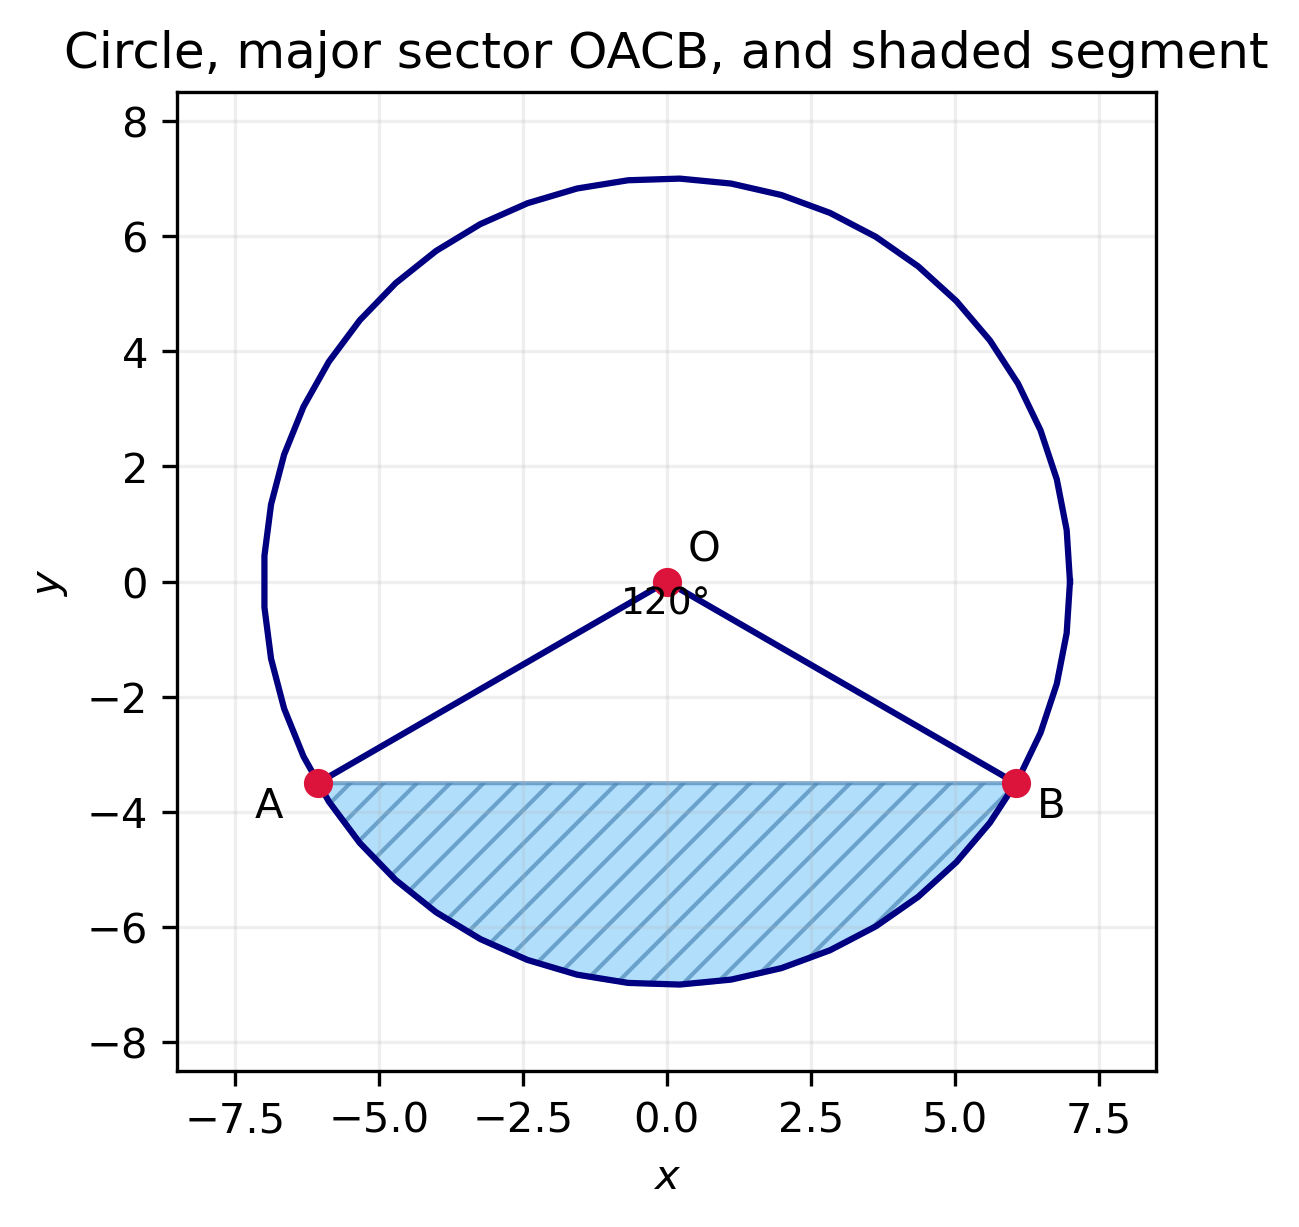
\includegraphics[width=0.47\linewidth]{figs/1.2.11.png}
    \caption{Major sector and shaded minor segment.}
\end{figure}

\item[1.2.12] A point $P(x,7)$ divides the line segment joining $A(-5,4)$ and $B(7,9)$ in a certain ratio. Find the ratio and hence find $x$.\nobreak\hfill\mbox{(10,2026)}



\vspace{0.6em}\par\solution


The vertical changes give $AP:PB=(7-4):(9-7)=3:2$. By the section formula, $x=\frac{3(7)+2(-5)}{3+2}=\frac{11}{5}$. The code plots $A$, $P$, and $B$.
\par\noindent\hfill\mbox{\textit{(\ref{formula-1-1-4})}}\par\begin{lstlisting}[frame=single, basicstyle=\rmfamily, escapeinside={(*@}{@*)}]
(*@\makebox[\dimexpr\linewidth-2\fboxsep-2\fboxrule\relax][c]{codes/1.2.12.py}@*)
\end{lstlisting}
\begin{figure}[H]
    \centering
    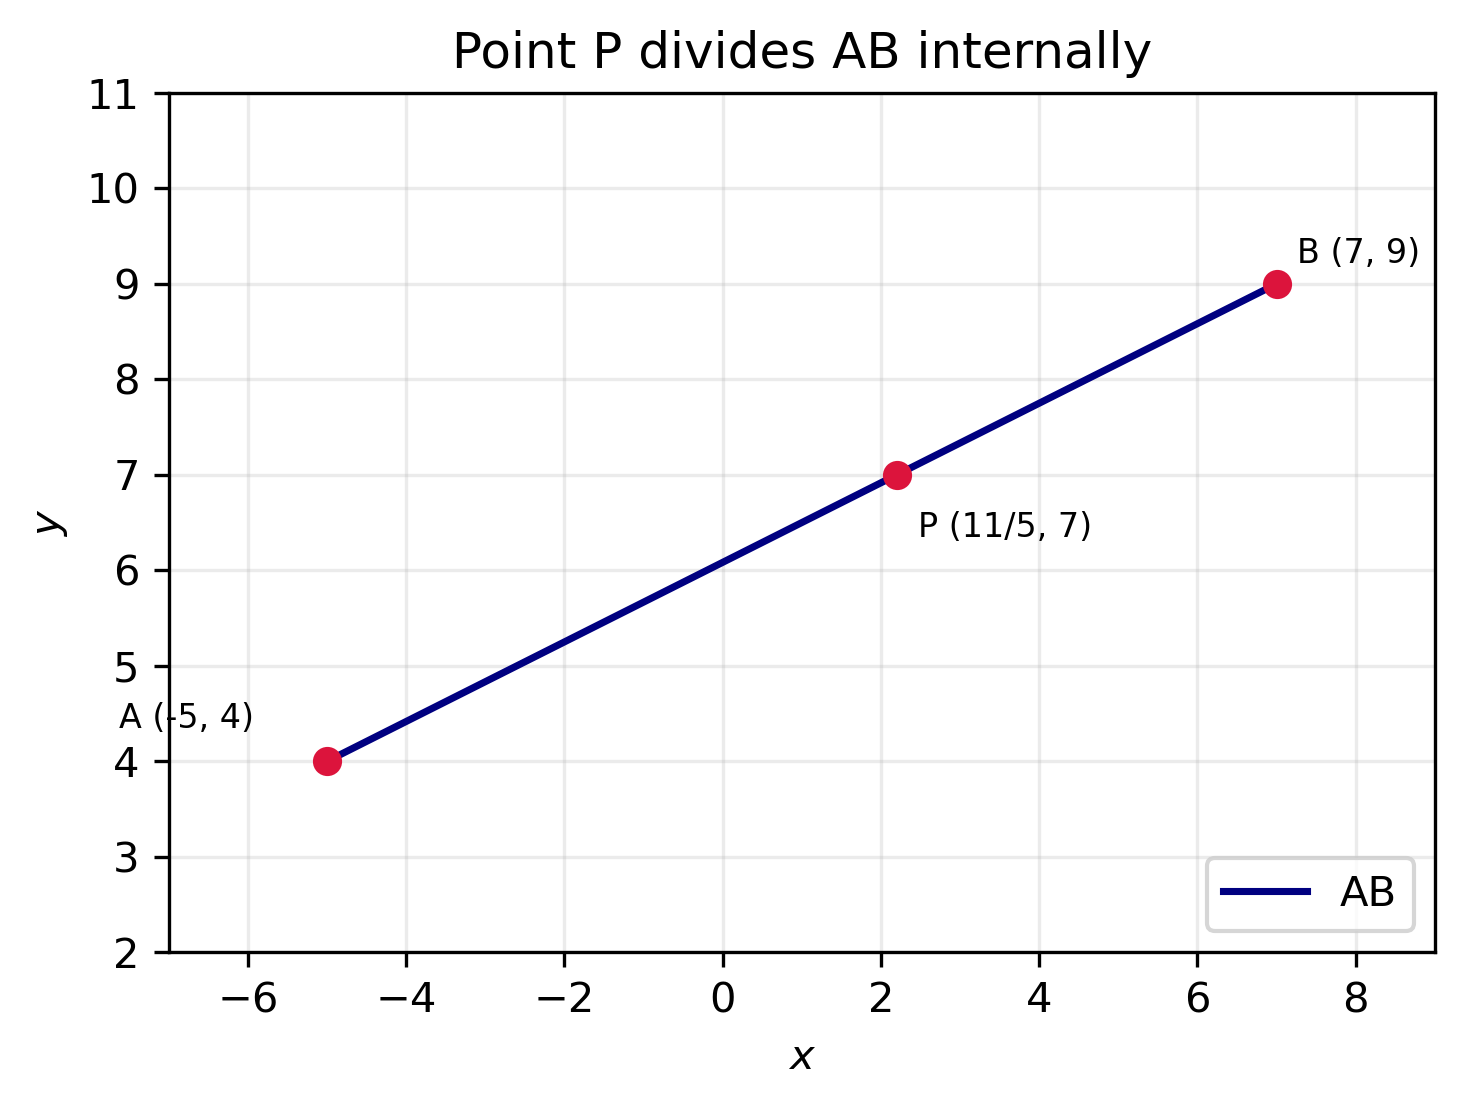
\includegraphics[width=0.52\linewidth]{figs/1.2.12.png}
    \caption{Point $P$ divides $AB$ internally in the ratio $3:2$.}
\end{figure}

\item[1.2.13] In the given figure, $PA$ is tangent to the circle with centre $O$, $OA=10$ cm, $AB=8$ cm, and $AB\perp OP$. Find $PB$.\nobreak\hfill\mbox{(10,2026)}



\vspace{0.6em}\par\solution


In right triangle $OAB$, $OB=\sqrt{10^2-8^2}=6$ cm. Let $PB=t$. Since $PA$ is tangent, $\triangle OAP$ is right-angled at $A$; also $\triangle PAB$ is right-angled at $B$. Thus $t^2+8^2=(t+6)^2-10^2$, giving $t=\frac{32}{3}$ cm. The code constructs this configuration and computes the length.
\par\noindent\hfill\mbox{\textit{(\ref{formula-1-1-2})}}\par\begin{lstlisting}[frame=single, basicstyle=\rmfamily, escapeinside={(*@}{@*)}]
(*@\makebox[\dimexpr\linewidth-2\fboxsep-2\fboxrule\relax][c]{codes/1.2.13.py}@*)
\end{lstlisting}
\begin{figure}[H]
    \centering
    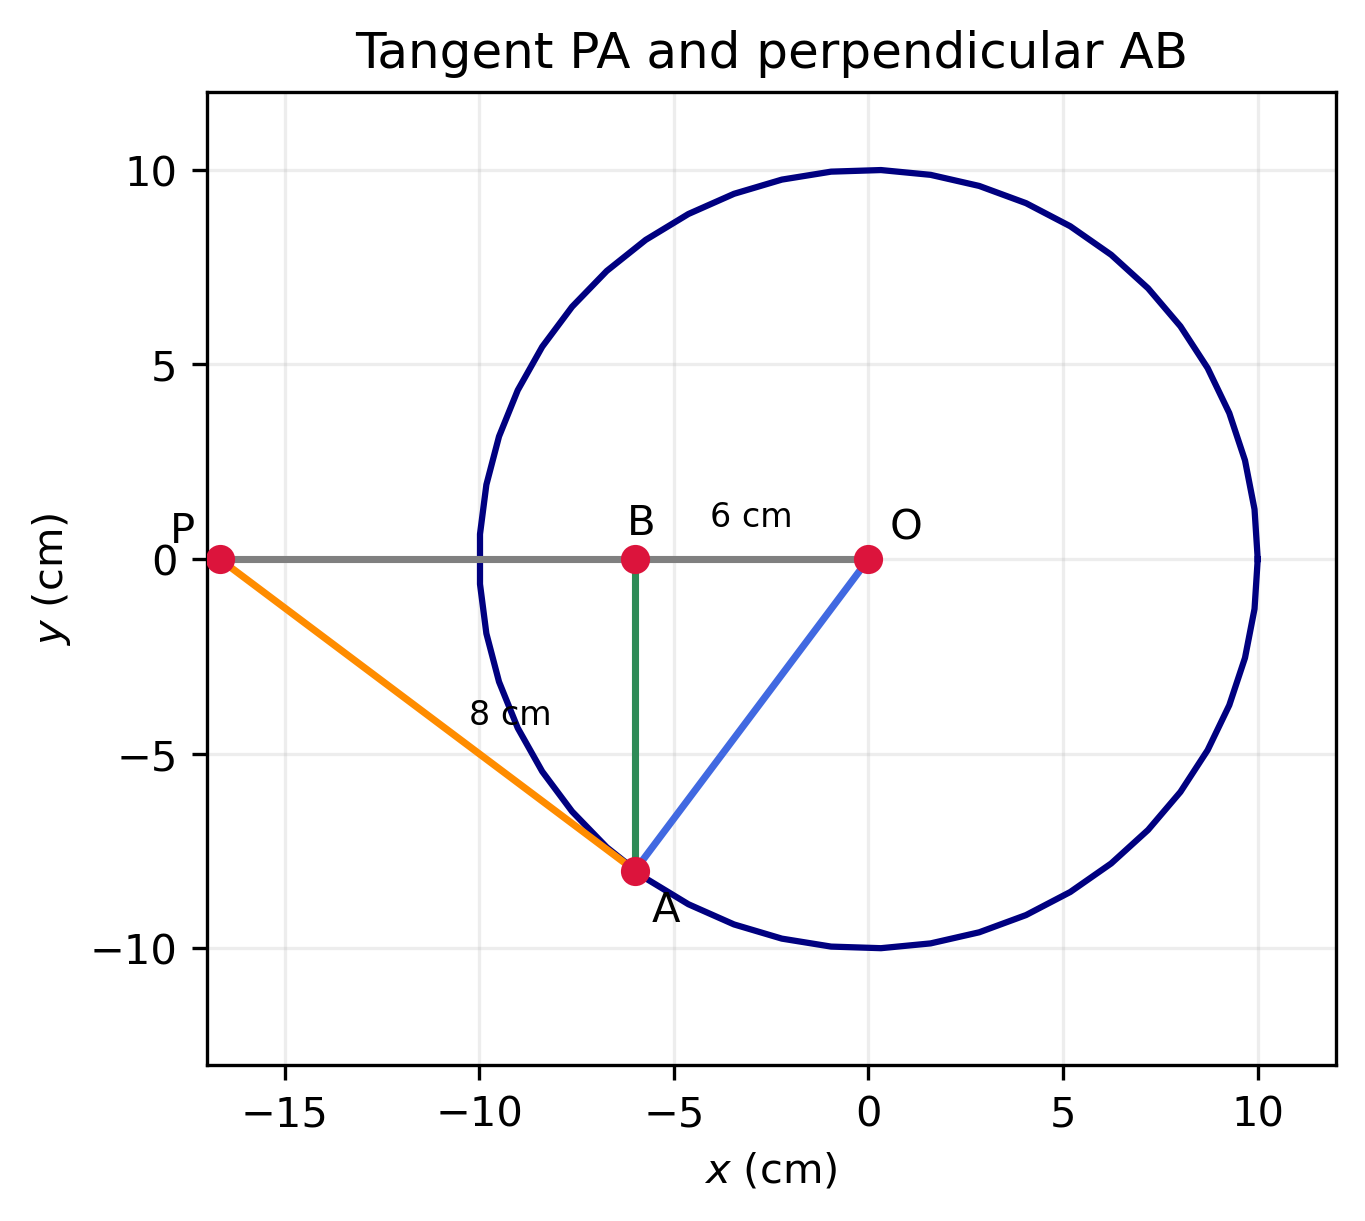
\includegraphics[width=0.50\linewidth]{figs/1.2.13.png}
    \caption{Tangent $PA$ and perpendicular segment $AB$.}
\end{figure}

\item[1.2.14] Solve graphically: $x-2y=3$, $3x-8y=7$.\nobreak\hfill\mbox{(10,2026)}



\vspace{0.6em}\par\solution

The two lines intersect at $(5,1)$, so the solution is $x=5$, $y=1$. The code plots both lines and marks their intersection; it uses the CoordGeo line-intersection function to calculate the point.
\begin{lstlisting}[frame=single, basicstyle=\rmfamily, escapeinside={(*@}{@*)}]
(*@\makebox[\dimexpr\linewidth-2\fboxsep-2\fboxrule\relax][c]{codes/1.2.14.py}@*)
\end{lstlisting}
\begin{figure}[H]
    \centering
    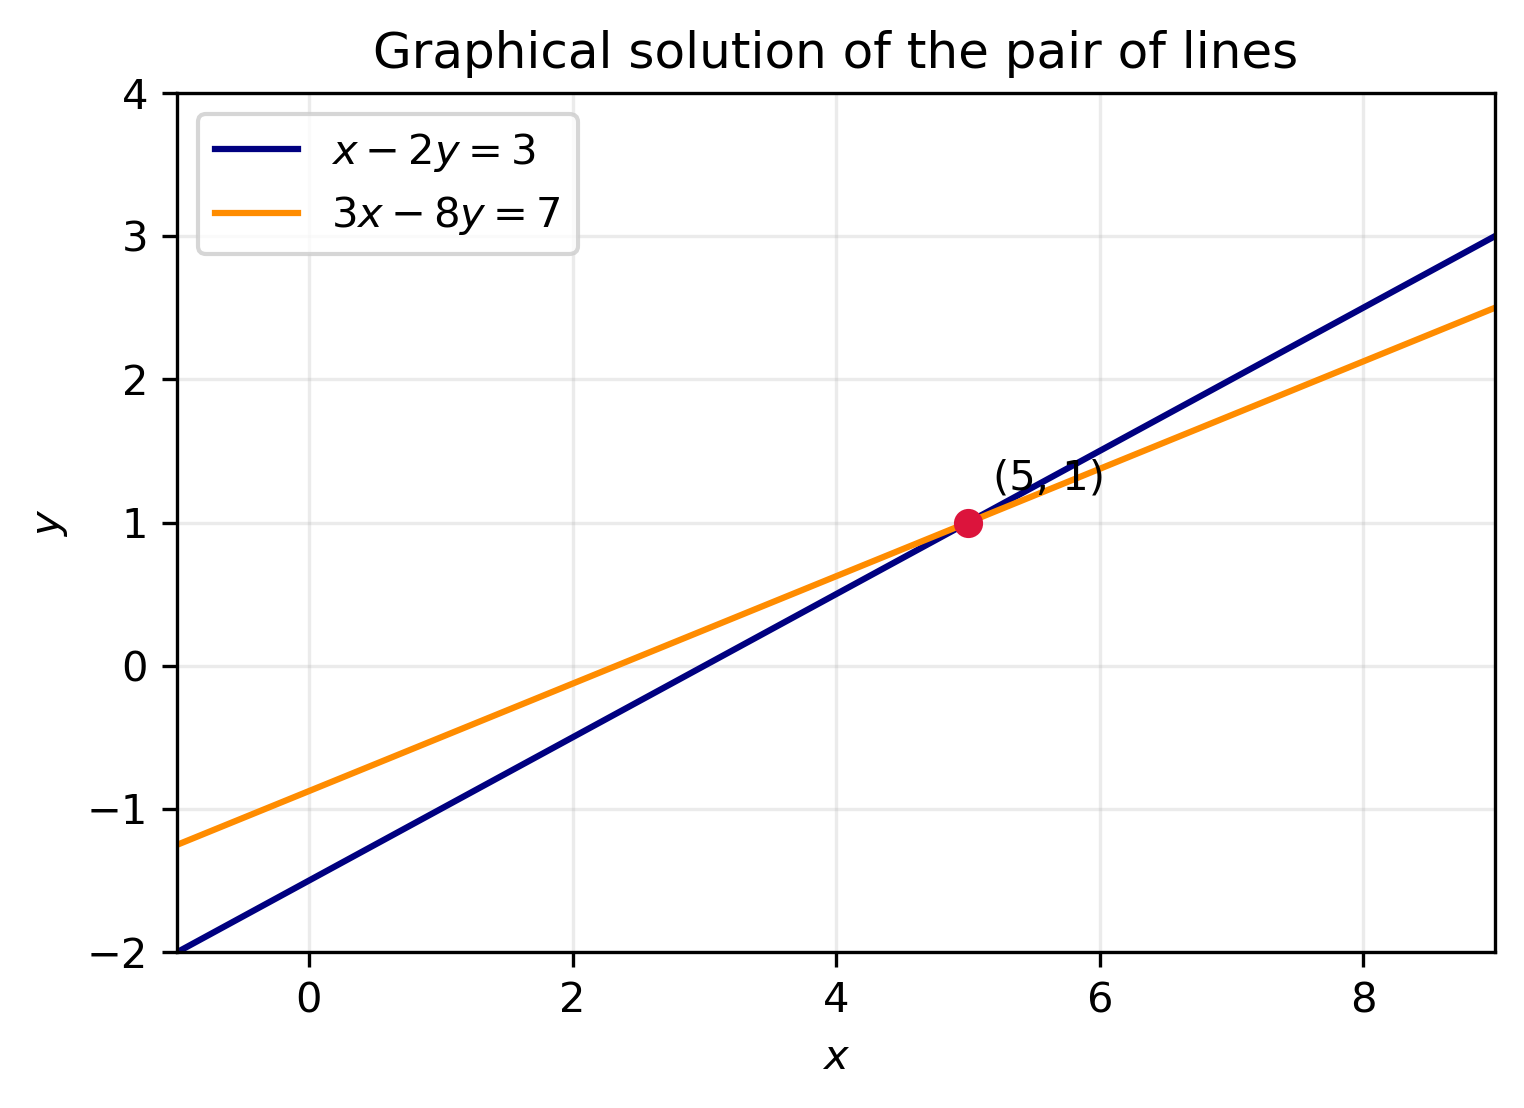
\includegraphics[width=0.52\linewidth]{figs/1.2.14.png}
    \caption{The lines intersect at $(5,1)$.}
\end{figure}

\item[1.2.15] A boy flies a kite with a $60$ m string at an elevation of $30^\circ$. Another boy on the roof of a $20$ m building sees the same kite at $45^\circ$. If the boys are on opposite sides of the kite, find the first boy's distance from the building and the kite's height from the ground. Use $\sqrt3=1.73$.\nobreak\hfill\mbox{(10,2026)}



\vspace{0.6em}\par\solution


Take the first boy as the origin, with horizontal and vertical unit vectors $\mathbf{i}$ and $\mathbf{j}$. The kite's position vector is
\[
\mathbf{k}=60(\cos30^\circ\,\mathbf{i}+\sin30^\circ\,\mathbf{j})=30\sqrt3\,\mathbf{i}+30\,\mathbf{j}.
\]
Thus its height above the ground is $30$ m. The rooftop is $20$ m high, so the kite is $10$ m above it. Since the rooftop boy sees the kite at $45^\circ$ and is on the opposite side, the rooftop position vector is
\[
\mathbf{r}=\mathbf{k}+10\mathbf{i}-10\mathbf{j}=(30\sqrt3+10)\mathbf{i}+20\mathbf{j}.
\]
Subtracting the building's vertical vector $20\mathbf{j}$ gives the building-base position vector $\mathbf{b}=(30\sqrt3+10)\mathbf{i}$. Therefore the first boy's distance from the building is $|\mathbf{b}|=30\sqrt3+10\approx61.9$ m, using $\sqrt3=1.73$. The code plots the configuration.
\par\noindent\hfill\mbox{\textit{(\ref{formula-1-1-7})}}\par\begin{lstlisting}[frame=single, basicstyle=\rmfamily, escapeinside={(*@}{@*)}]
(*@\makebox[\dimexpr\linewidth-2\fboxsep-2\fboxrule\relax][c]{codes/1.2.15.py}@*)
\end{lstlisting}
\begin{figure}[H]
    \centering
    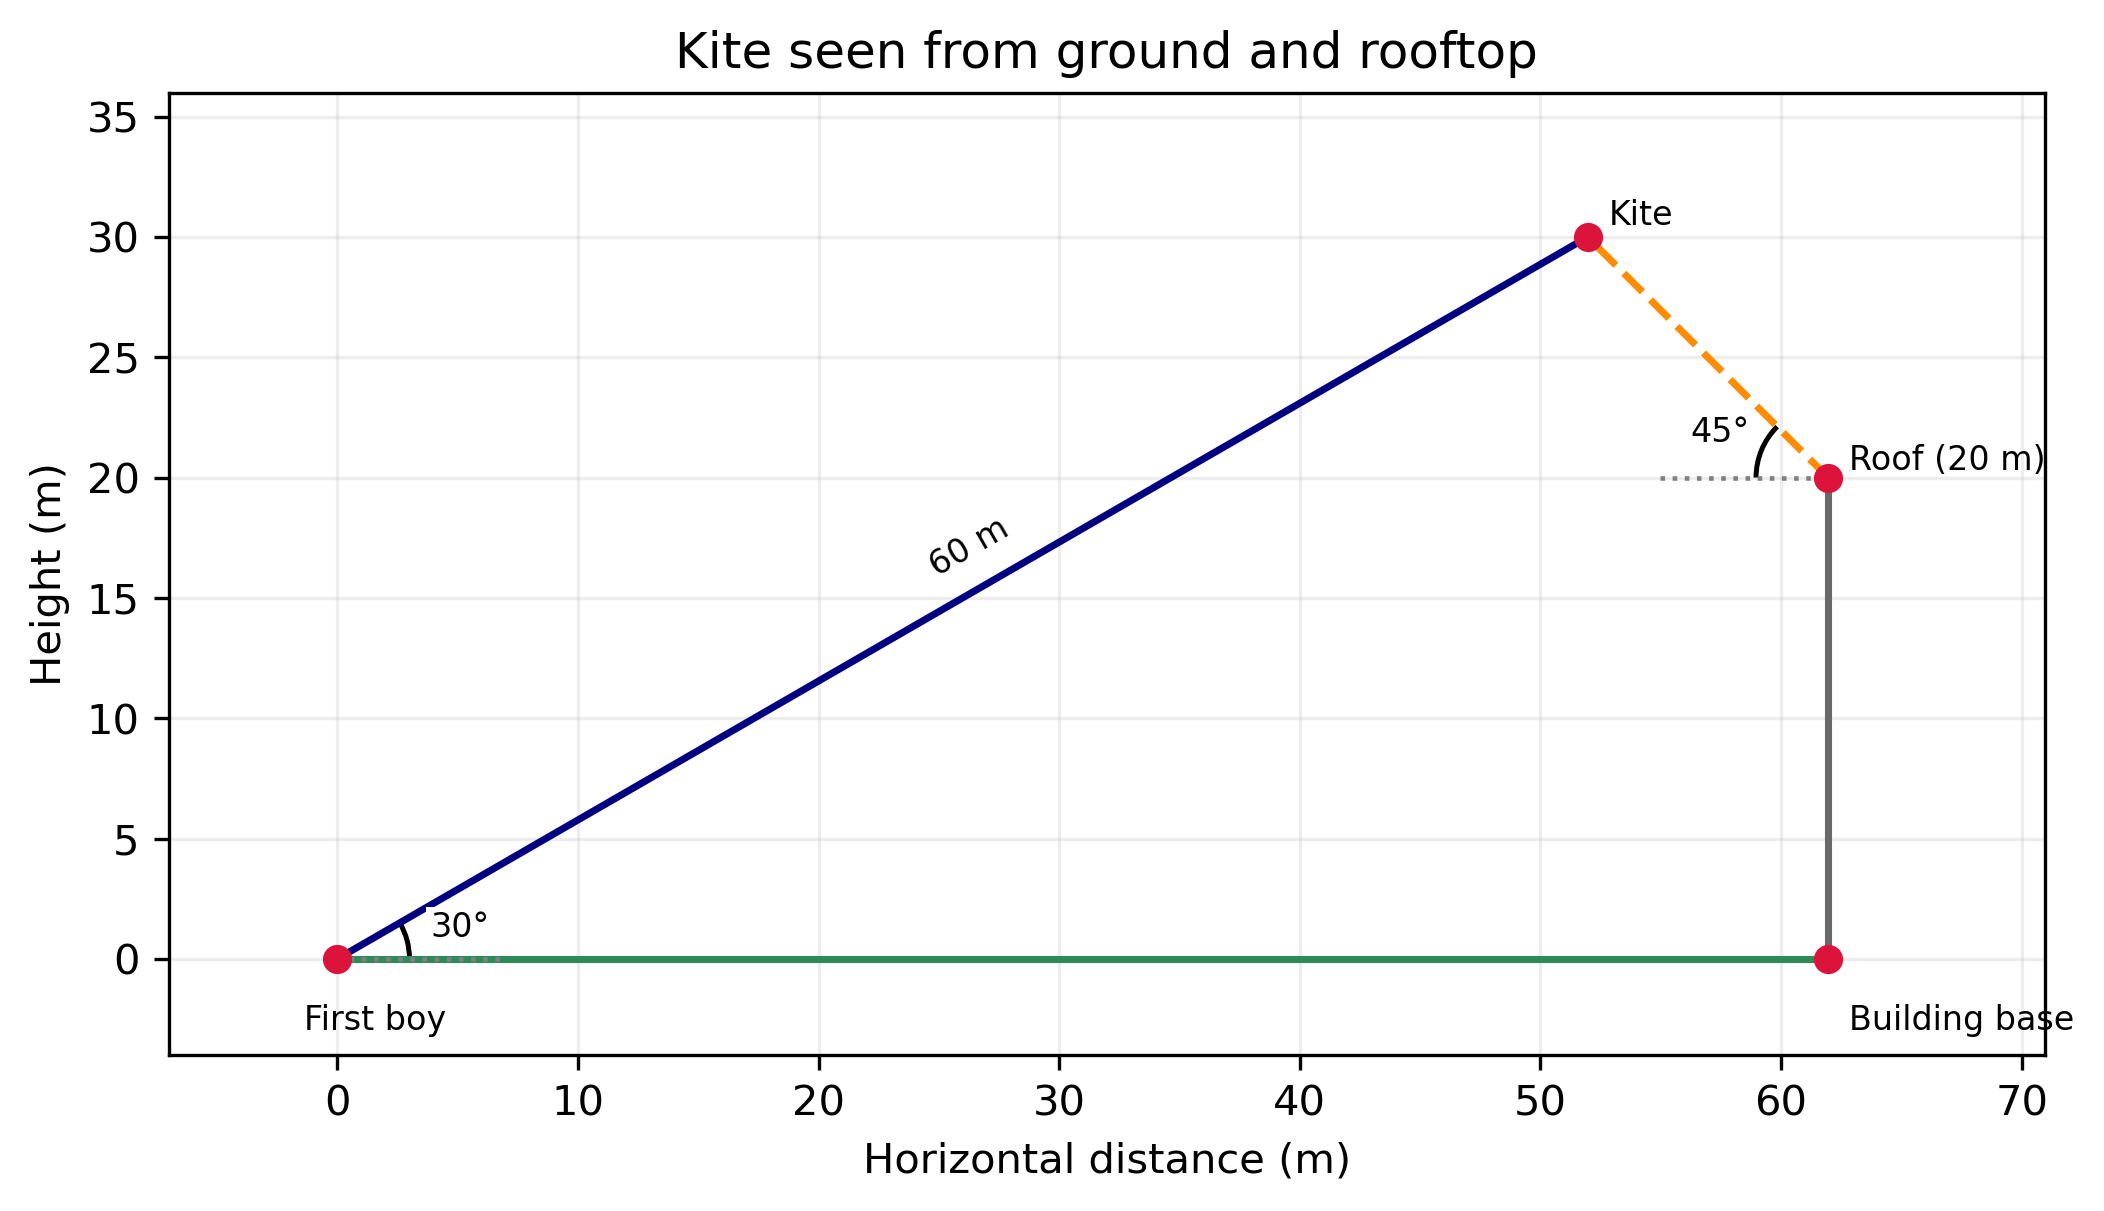
\includegraphics[width=0.58\linewidth]{figs/1.2.15.png}
    \caption{Kite position relative to the two observers.}
\end{figure}

\item[1.2.16] The arch is modelled by $p(x)=-x^2+2x+8$, where $x$ is distance along the stage. Find (i) its height, (ii)(a) its zeroes and the corresponding graph points, or (ii)(b) its span, and (iii) the point where it meets the $y$-axis.\nobreak\hfill\mbox{(10,2026)}



\vspace{0.6em}\par\solution


Writing $p(x)=-(x-1)^2+9$ shows the maximum height is $9$ ft. Factoring gives $p(x)=-(x-4)(x+2)$, so the zeroes are $-2$ and $4$, represented by $(-2,0)$ and $(4,0)$. The span between these intercepts is $6$ ft. At $x=0$, $p(0)=8$, so the $y$-intercept is $(0,8)$.
\par\noindent\hfill\mbox{\textit{(\ref{formula-1-1-1})}}\par
The C program uses Newton--Raphson to find the roots and solve $p'(x)=0$ for the vertex:
\par\noindent\hfill\mbox{\textit{(\ref{formula-1-1-11})}}\par\begin{lstlisting}[frame=single, basicstyle=\rmfamily, escapeinside={(*@}{@*)}]
(*@\makebox[\dimexpr\linewidth-2\fboxsep-2\fboxrule\relax][c]{codes/1.2.16.c}@*)
\end{lstlisting}
The Python program plots the parabola and marks these points:
\begin{lstlisting}[frame=single, basicstyle=\rmfamily, escapeinside={(*@}{@*)}]
(*@\makebox[\dimexpr\linewidth-2\fboxsep-2\fboxrule\relax][c]{codes/1.2.16.py}@*)
\end{lstlisting}
\begin{figure}[H]
    \centering
    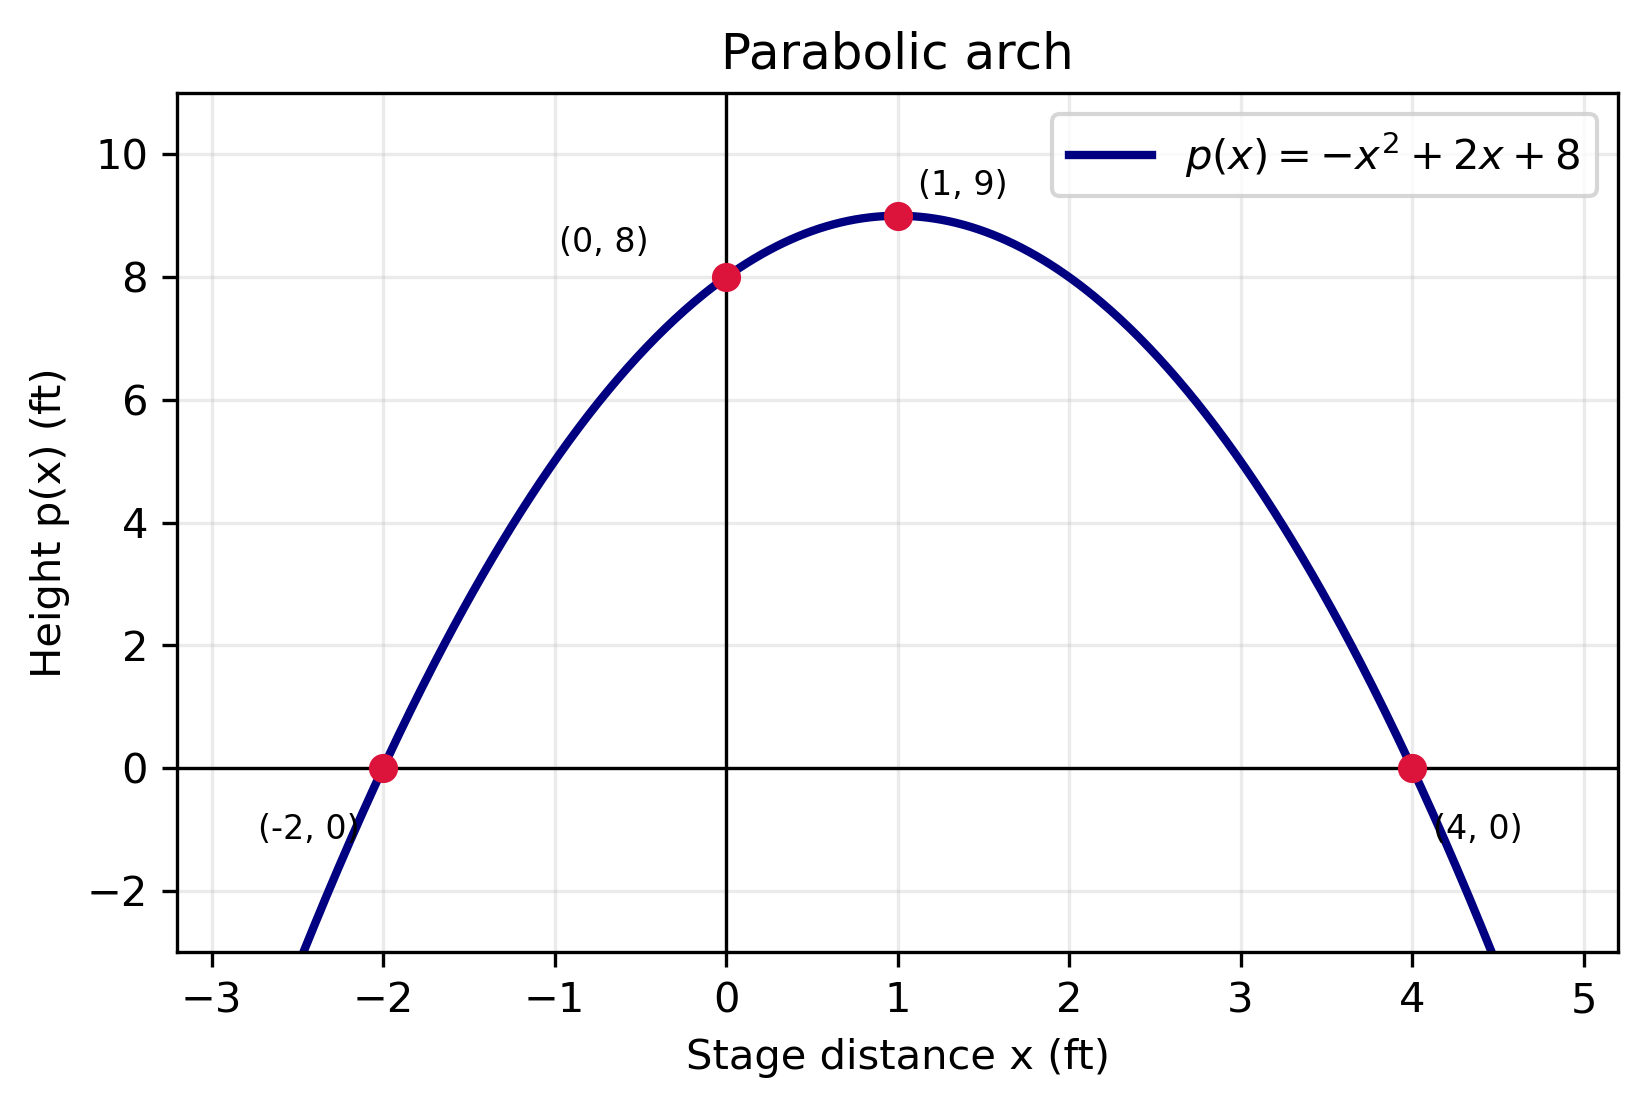
\includegraphics[width=0.56\linewidth]{figs/1.2.16.png}
    \caption{The arch polynomial and its intercepts and vertex.}
\end{figure}

\item[1.2.17] Three cards are dropped from two identical packs: a queen of hearts, a ten of spades, and an ace of clubs. One of the remaining cards is drawn at random. Find (i) the probability of a face card, (ii) the probability of a king or queen, (iii)(a) whether the probability of a queen would be higher if no cards were dropped, or (iii)(b) the probability of a jack and compare it with the probability when no cards were dropped.\nobreak\hfill\mbox{(10,2026)}



\vspace{0.6em}\par\solution


After the drops, $101$ cards remain. Let $X$ be the drawn card's rank category ($K$, $Q$, $J$, or Other). Its PMF with and without the drops is:
\[\begingroup\renewcommand{\arraystretch}{1.25}
\begin{array}{c|cccc}
&K&Q&J&\text{Other}\\\hline
p_X(x)\text{ after drops}&\frac{8}{101}&\frac{7}{101}&\frac{8}{101}&\frac{78}{101}\\
p_X(x)\text{ with no drops}&\frac{8}{104}&\frac{8}{104}&\frac{8}{104}&\frac{80}{104}
\end{array}\endgroup
\]
\par\noindent\hfill\mbox{\textit{(\ref{formula-1-1-9})}}\par
(i) $P(\text{face card})=\frac{8+7+8}{101}=\frac{23}{101}$. (ii) $P(K\text{ or }Q)=\frac{8+7}{101}=\frac{15}{101}$.

(iii)(a) $\frac{7}{101}<\frac{8}{104}$, so queens are more likely with no drops. (iii)(b) $\frac{8}{101}>\frac{8}{104}$; since no jack was removed, jacks are more likely after the drops.

\end{enumerate}

\clearpage

\section{Class 12}
\subsection{Formulae}
\renewcommand{\paperlabelprefix}{12-65-3-1}
\begin{enumerate}[label=\normalfont 2.1.\arabic*.,ref=2.1.\arabic*]
\setlength{\itemsep}{0.35em}
\item \label{formula-2-1-1} \textbf{Matrix products and inverses.} If $A$ is $m\times n$ and $B$ is $n\times p$, then $AB$ is $m\times p$. For a square nonsingular matrix,
\begin{equation*}\tag{2.1.1.1}
A^{-1}=\frac{\operatorname{adj}A}{\det A},\qquad A\operatorname{adj}A=(\det A)I.
\end{equation*}
\item \label{formula-2-1-2} \textbf{Inverse from a matrix identity.} If $A^2+\alpha A+\beta I=0$ and $\beta\ne0$, then $A^{-1}=-(A+\alpha I)/\beta$.
\item \label{formula-2-1-3} \textbf{Continuity, derivatives, and extrema.} $f$ is continuous at $a$ when $\lim_{x\to a}f(x)=f(a)$. At an interior local extremum of a differentiable function, $f\prime(a)=0$. The derivative is $f'(a)=\lim_{h\to0}\frac{f(a+h)-f(a)}h$; the chain rule is $\frac{d}{dx}F(g(x))=F'(g(x))g'(x)$.
\item \label{formula-2-1-4} \textbf{Useful derivatives.}
\begin{equation*}\tag{2.1.4.1}
\frac{d}{dx}\tan x=\sec^2x,\qquad
\frac{d}{dx}\ln x=\frac1x,\qquad
\frac{d}{dx}e^x=e^x.
\end{equation*}
\item \label{formula-2-1-5} \textbf{Useful integrals.}
\begin{equation*}\tag{2.1.5.1}
\int\frac{dx}{a^2+x^2}=\frac1a\tan^{-1}\!\frac xa+C,\qquad
\int\frac{dx}{\sqrt{a^2-x^2}}=\sin^{-1}\!\frac xa+C.
\end{equation*}
For the exponential form used in the paper, $\int\frac{dx}{2^x+2^{-x}}=\frac{\tan^{-1}(2^x)}{\ln2}+C$. If $f(x)\ge0$, the area under $y=f(x)$ from $a$ to $b$ is $\int_a^b f(x)\,dx$.
\item \label{formula-2-1-6} \textbf{Symmetry in definite integrals.} If $f$ is even, $\int_{-a}^{a}f(x)\,dx=2\int_0^a f(x)\,dx$. If $f(x)+f(\pi/2-x)=1$ on $[0,\pi/2]$, then $\int_0^{\pi/2}f(x)\,dx=\pi/4$.
\item \label{formula-2-1-7} \textbf{Homogeneous differential equations.} For $dy/dx=F(y/x)$, use $y=vx$, so $dy/dx=v+x\,dv/dx$; the resulting equation is separable.
\item \label{formula-2-1-8} \textbf{Probability.}
\begin{equation*}\tag{2.1.8.1}
P(A\cup B)=P(A)+P(B)-P(A\cap B),\quad
P(A\mid B)=\frac{P(A\cap B)}{P(B)}.
\end{equation*}
For independent events, $P(A\cap B)=P(A)P(B)$.
\item \label{formula-2-1-9} \textbf{Vectors.} $\vec a\cdot\vec b=|\vec a||\vec b|\cos\theta$; perpendicular nonzero vectors have $\vec a\cdot\vec b=0$. Also, $(\vec a+\vec b)\cdot(\vec a-\vec b)=|\vec a|^2-|\vec b|^2$. Triangle area is $\frac12|\vec a\times\vec b|$ for two side vectors.
\item \label{formula-2-1-10} \textbf{Linear programming.} A linear objective reaches its maximum or minimum at a vertex of the feasible region; evaluate the objective at every feasible vertex.
\item \label{formula-2-1-11} \textbf{Lines and distance in 3D.} A line through $\vec a$ with direction $\vec d$ is $\vec r=\vec a+t\vec d$. Two direction vectors are perpendicular when $\vec d_1\cdot\vec d_2=0$. To find the perpendicular component of a vector $\vec v$ to a nonzero direction $\vec d$, use $\vec v_\perp=\vec v-\frac{\vec v\cdot\vec d}{\vec d\cdot\vec d}\vec d$. For skew lines with direction vectors $\vec d_1,\vec d_2$ through $\vec a_1,\vec a_2$,
\begin{equation*}\tag{2.1.11.1}
d=\frac{|(\vec a_2-\vec a_1)\cdot(\vec d_1\times\vec d_2)|}{|\vec d_1\times\vec d_2|}.
\end{equation*}
\item \label{formula-2-1-12} \textbf{Bayes' theorem.} $P(A_i\mid B)=\frac{P(B\mid A_i)P(A_i)}{\sum_jP(B\mid A_j)P(A_j)}$ for a partition $\{A_j\}$.
\item \label{formula-2-1-13} \textbf{Eigenvalues of matrix polynomials.} If $Av=\lambda v$ for $v\ne0$ and $q(A)=0$, then $q(\lambda)=0$.
\item \label{formula-2-1-14} \textbf{Idempotent matrices.} If $A^2=A$, then $A$ is diagonalizable with eigenvalues $0$ and $1$; in a suitable basis, $A=\operatorname{diag}(I_r,0)$, where $r=\operatorname{rank}(A)$.
\item \label{formula-2-1-15} \textbf{Squeeze theorem.} If $g(x)\le f(x)\le h(x)$ near $a$ and $\lim_{x\to a}g(x)=\lim_{x\to a}h(x)=L$, then $\lim_{x\to a}f(x)=L$.
\item \label{formula-2-1-16} \textbf{Composite trapezoidal rule.} For $x_k=a+kh$, $h=(b-a)/n$,
\begin{equation*}\tag{2.1.16.1}
\begin{aligned}
T_n=A_n&=\frac h2\left[f(x_0)+2\sum_{k=1}^{n-1}f(x_k)+f(x_n)\right],\\
A_0&=0,\qquad A_{k+1}-A_k=\frac h2\bigl(f(x_k)+f(x_{k+1})\bigr).
\end{aligned}
\end{equation*}
This rule is exact on subintervals where $f$ is linear.
\item \label{formula-2-1-17} \textbf{Area accumulation by a difference equation.} For $x_k=a+kh$, $h=(b-a)/n$, choose $\xi_k\in[x_k,x_{k+1}]$, let $A_0=0$, and set $A_{k+1}-A_k=hf(\xi_k)$. Then
\begin{equation*}\tag{2.1.17.1}
A_n=h\sum_{k=0}^{n-1}f(\xi_k),\qquad \int_a^b f(x)\,dx=\lim_{n\to\infty}A_n
\end{equation*}
when $f$ is continuous on $[a,b]$.
\item \label{formula-2-1-18} \textbf{Derivative test for monotonicity.} If $f'(x)>0$ throughout an interval, then $f$ is strictly increasing there; if $f'(x)<0$ throughout, then $f$ is strictly decreasing there.
\item \label{formula-2-1-19} \textbf{Gram matrix.} For vectors $v_1,\ldots,v_m$, the Gram matrix is $G_{ij}=v_i\cdot v_j$. For $v=\sum_i c_i v_i$, $|v|^2=c^{\mathsf T}Gc$; in particular, $G$ is positive semidefinite.
\item \label{formula-2-1-20} \textbf{Discrete PMF and binomial distribution.} A PMF satisfies $p_X(x)=P(X=x)$ and $\sum_xp_X(x)=1$; joint PMFs marginalize by summation, and $p_{X,Y}(x,y)=P(X=x)P(Y=y\mid X=x)$. For $X\sim\operatorname{Binomial}(n,p)$,
\begin{equation*}\tag{2.1.20.1}
p_X(k)=\binom nkp^k(1-p)^{n-k},\qquad k=0,1,\ldots,n.
\end{equation*}
\item \label{formula-2-1-21} \textbf{Gaussian elimination.} Apply elementary row operations to the augmented matrix $[A\mid b]$ to obtain an equivalent system. If $A$ is nonsingular, the reduced system has a unique solution.
\end{enumerate}

\subsection{Solved Questions}
\renewcommand{\paperlabelprefix}{12-65-3-1}
\graphicspath{{12/}}
\begin{enumerate}[label={},font=\normalfont,leftmargin=1.15cm,labelwidth=1.0cm,labelsep=0.15cm,itemindent=0pt,listparindent=0pt,itemsep=\baselineskip,parsep=0pt,topsep=0pt]
\item[2.2.1] If $A^2=4A+3I$ and $A^{-1}=xA+yI$, find $x+y$.

\begin{multicols}{4}
\begin{enumerate}
\setlength{\itemsep}{0pt}
    \item $-1$
    \item $1$
    \item $\frac53$
    \item $7$\nobreak\hfill\mbox{(12,2026)}
\end{enumerate}
\end{multicols}



\vspace{0.6em}\par\solution


Let $v\ne0$ be an eigenvector of $A$ with eigenvalue $\lambda$. Applying $A^2=4A+3I$ to $v$ gives $\lambda^2-4\lambda-3=0$, so the possible eigenvalues are $\lambda_+=2+\sqrt7$ and $\lambda_-=2-\sqrt7$.
\par\noindent\hfill\mbox{\textit{(\ref{formula-2-1-13})}}\par
They are distinct. For the intended non-scalar case, both occur. Applying $A^{-1}=xA+yI$ to eigenvectors for these eigenvalues gives
\[
\frac1{\lambda_+}=x\lambda_++y,\qquad \frac1{\lambda_-}=x\lambda_-+y.
\]
The eigenvalue equation also gives $1/\lambda_\pm=(\lambda_\pm-4)/3$. Subtracting the two equations yields
\[
x=\frac{1/\lambda_+-1/\lambda_-}{\lambda_+-\lambda_-}=\frac13,\qquad y=\frac1{\lambda_+}-x\lambda_+=-\frac43.
\]
Therefore, $x+y=-1$, so the correct answer is \textbf{a)}.

\textit{If $A$ is a scalar multiple of $I$, the values of $x$ and $y$ are not uniquely determined; the question implicitly assumes the non-scalar case.}
\item[2.2.2] If a square matrix $A$ satisfies $A^2=A$ and $(I-A)^3=xA+I$, find $x$.\nobreak\hfill\mbox{(12,2026)}



\vspace{0.6em}\par\solution


Since $A^2=A$, its minimal polynomial divides $t(t-1)$, which has distinct roots; hence $A$ is diagonalizable. For some invertible matrix $P$, write
\[
A=P\begin{bmatrix}I_r&0\\0&0\end{bmatrix}P^{-1},\qquad I-A=P\begin{bmatrix}0&0\\0&I_{n-r}\end{bmatrix}P^{-1}.
\]
\par\noindent\hfill\mbox{\textit{(\ref{formula-2-1-14})}}\par
Thus $(I-A)^3=P\begin{bmatrix}0&0\\0&I_{n-r}\end{bmatrix}P^{-1}=I-A$. Comparing with $xA+I$ gives $(x+1)A=0$, so for $A\ne0$, $\boxed{x=-1}$. If $A=0$, the equation holds for every $x$; the stated answer assumes $A$ is nonzero.

\item[2.2.3] If $B(\operatorname{adj}B)=\begin{bmatrix}\frac13&0&0\\0&\frac13&0\\0&0&\frac13\end{bmatrix}$, find $\det(B^{-1})$.

\begin{multicols}{4}
\begin{enumerate}
\setlength{\itemsep}{0pt}
    \item $\frac13$
    \item $3$
    \item $-3$
    \item $9$\nobreak\hfill\mbox{(12,2026)}
\end{enumerate}
\end{multicols}



\vspace{0.6em}\par\solution


Since $B(\operatorname{adj}B)=\frac13I_3$ is nonsingular, $B$ is nonsingular. Let $v\ne0$ be an eigenvector of $B$ with eigenvalue $\lambda$. Then $\lambda\ne0$ and, using $\operatorname{adj}B=\det(B)B^{-1}$,
\[
\operatorname{adj}B\,v=\frac{\det(B)}{\lambda}v,\qquad B(\operatorname{adj}B)v=\det(B)v.
\]
But the given equation also gives $B(\operatorname{adj}B)v=\frac13v$. Since $v\ne0$, $\det(B)=\frac13$, and hence $\det(B^{-1})=\frac1{\det(B)}=\boxed{3}$, option \textbf{b)}. The Python code checks the determinant value from the given product.
\par\noindent\hfill\mbox{\textit{(\ref{formula-2-1-1})}}\par\begin{lstlisting}[frame=single, basicstyle=\rmfamily, escapeinside={(*@}{@*)}]
(*@\makebox[\dimexpr\linewidth-2\fboxsep-2\fboxrule\relax][c]{codes/2.2.3.py}@*)
\end{lstlisting}

\item[2.2.4] Find $k$ such that $f(x)=\begin{cases}x^2\sin(1/x),&x\ne0,\\k(x+1),&x=0\end{cases}$ is continuous.\nobreak\hfill\mbox{(12,2026)}



\vspace{0.6em}\par\solution


At $x=0$, the second branch gives $f(0)=k$. For $x\ne0$, since $-1\le\sin(1/x)\le1$ and $x^2\ge0$,
\[
-x^2\le x^2\sin(1/x)\le x^2.
\]
Both bounds tend to $0$ as $x\to0$. By the squeeze theorem, $\lim_{x\to0}x^2\sin(1/x)=0$. Thus continuity requires $k=0$. The figure plots the function together with the bounding curves $y=-x^2$ and $y=x^2$.
\par\noindent\hfill\mbox{\textit{(\ref{formula-2-1-3}, \ref{formula-2-1-15})}}\par\begin{lstlisting}[frame=single, basicstyle=\rmfamily, escapeinside={(*@}{@*)}]
(*@\makebox[\dimexpr\linewidth-2\fboxsep-2\fboxrule\relax][c]{codes/2.2.4.py}@*)
\end{lstlisting}
\begin{figure}[H]\centering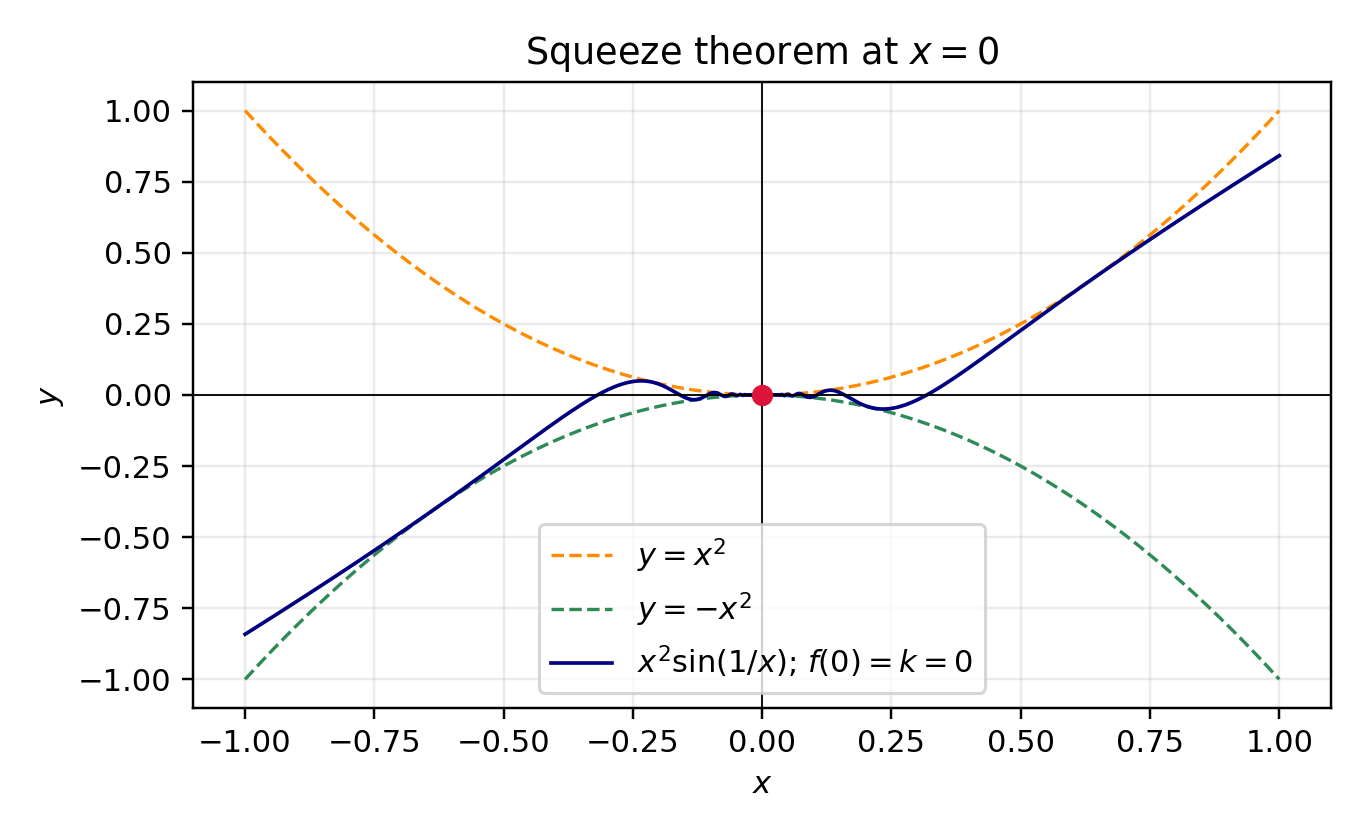
\includegraphics[width=0.68\linewidth]{figs/2.2.4.png}\caption{The function approaches $0$ as $x$ approaches $0$.}\end{figure}

\item[2.2.5] Evaluate $\int_{-1}^{1}(1-|x|)\,dx$ by identifying the matching option:

\begin{multicols}{2}
\begin{enumerate}
\setlength{\itemsep}{0pt}
    \item $2\int_0^1(1+x)\,dx$
    \item $2\int_{-1}^0(1+x)\,dx$
    \item $0$
    \item $2\int_{-1}^0(1-x)\,dx$\nobreak\hfill\mbox{(12,2026)}
\end{enumerate}
\end{multicols}



\vspace{0.6em}\par\solution


Use the nodes $x_0=-1$, $x_1=0$, and $x_2=1$ ($h=1$), where the function values are $0$, $1$, and $0$. The composite trapezoidal rule gives
\[
T=\frac{h}{2}\bigl(f(x_0)+2f(x_1)+f(x_2)\bigr)
=\frac12(0+2+0)=1.
\]
This is exact because $f(x)=1-|x|$ is linear on each half of the interval.

The same area accumulation can be written as a difference equation. Let $A_j$ be the accumulated area through $x_j$, with $A_0=0$. For $j=0,1$,
\[
A_{j+1}-A_j=\frac{h}{2}\bigl(f(x_j)+f(x_{j+1})\bigr).
\]
Thus $A_1-A_0=\frac12$ and $A_2-A_1=\frac12$, giving $A_2=1$. Also, on $[-1,0]$, $f(x)=1+x$; by symmetry the integral is $2\int_{-1}^0(1+x)\,dx$, which is option \textbf{b)}.\par\noindent\hfill\mbox{\textit{(\ref{formula-2-1-6}, \ref{formula-2-1-16})}}\par\begin{lstlisting}[frame=single, basicstyle=\rmfamily, escapeinside={(*@}{@*)}]
(*@\makebox[\dimexpr\linewidth-2\fboxsep-2\fboxrule\relax][c]{codes/2.2.5.py}@*)
\end{lstlisting}
\begin{figure}[H]\centering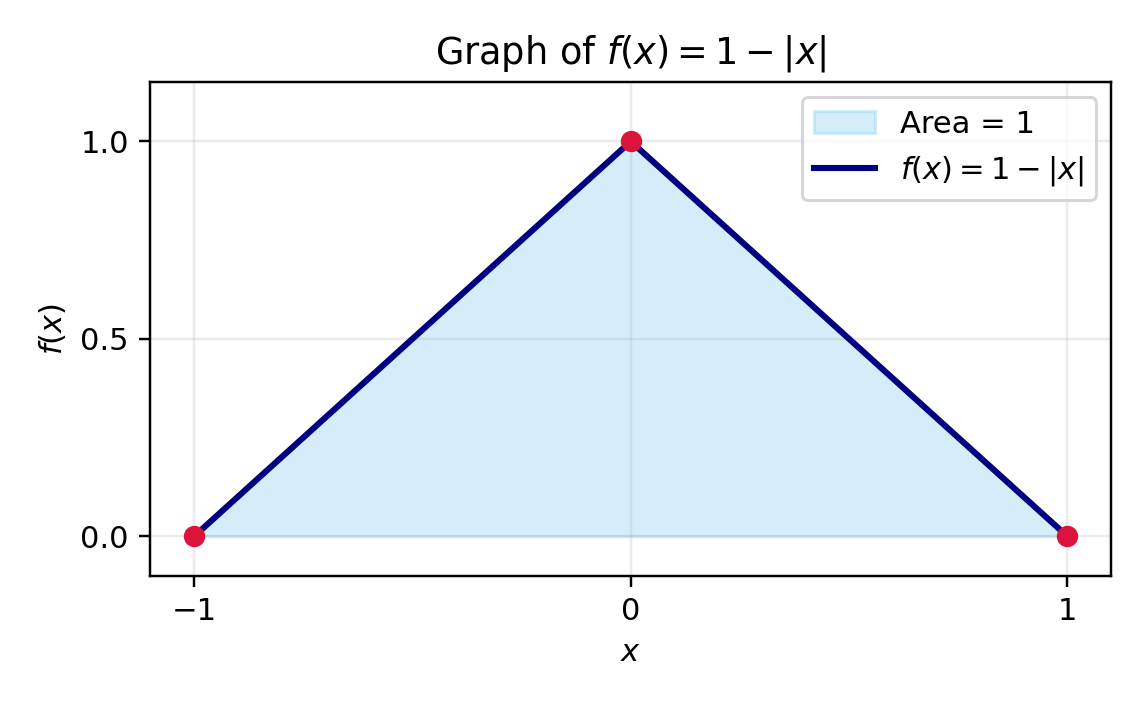
\includegraphics[width=0.40\linewidth]{figs/2.2.5.png}\caption{Graph of $f(x)=1-|x|$ on $[-1,1]$.}\end{figure}

\item[2.2.6] For the circle $x^2+y^2=9$, identify the integral for the shaded cap above $y=1$.

\begin{multicols}{2}
\begin{enumerate}
\setlength{\itemsep}{0pt}
    \item $\int_1^3\sqrt{9-y^2}\,dy$
    \item $2\int_1^3\sqrt{9-y^2}\,dy$
    \item $\int_0^3\sqrt{9-x^2}\,dx$
    \item $2\int_0^3\sqrt{9-x^2}\,dx$\nobreak\hfill\mbox{(12,2026)}
\end{enumerate}
\end{multicols}



\vspace{0.6em}\par\solution


At height $y$, the cap's width is $w(y)=2\sqrt{9-y^2}$ for $1\le y\le3$. Thus $A=\int_1^3w(y)\,dy$, which is option \textbf{b)}. CVXPY approximates this area with midpoint slices by maximizing $\Delta y\sum_iw_i$ subject to $0\le w_i\le2\sqrt{9-y_i^2}$; the code compares the result with all four choices.\par\noindent\hfill\mbox{\textit{(\ref{formula-2-1-5}, \ref{formula-2-1-10}, \ref{formula-2-1-17})}}\par\begin{lstlisting}[frame=single, basicstyle=\rmfamily, escapeinside={(*@}{@*)}]
(*@\makebox[\dimexpr\linewidth-2\fboxsep-2\fboxrule\relax][c]{codes/2.2.6.py}@*)
\end{lstlisting}
\begin{figure}[H]\centering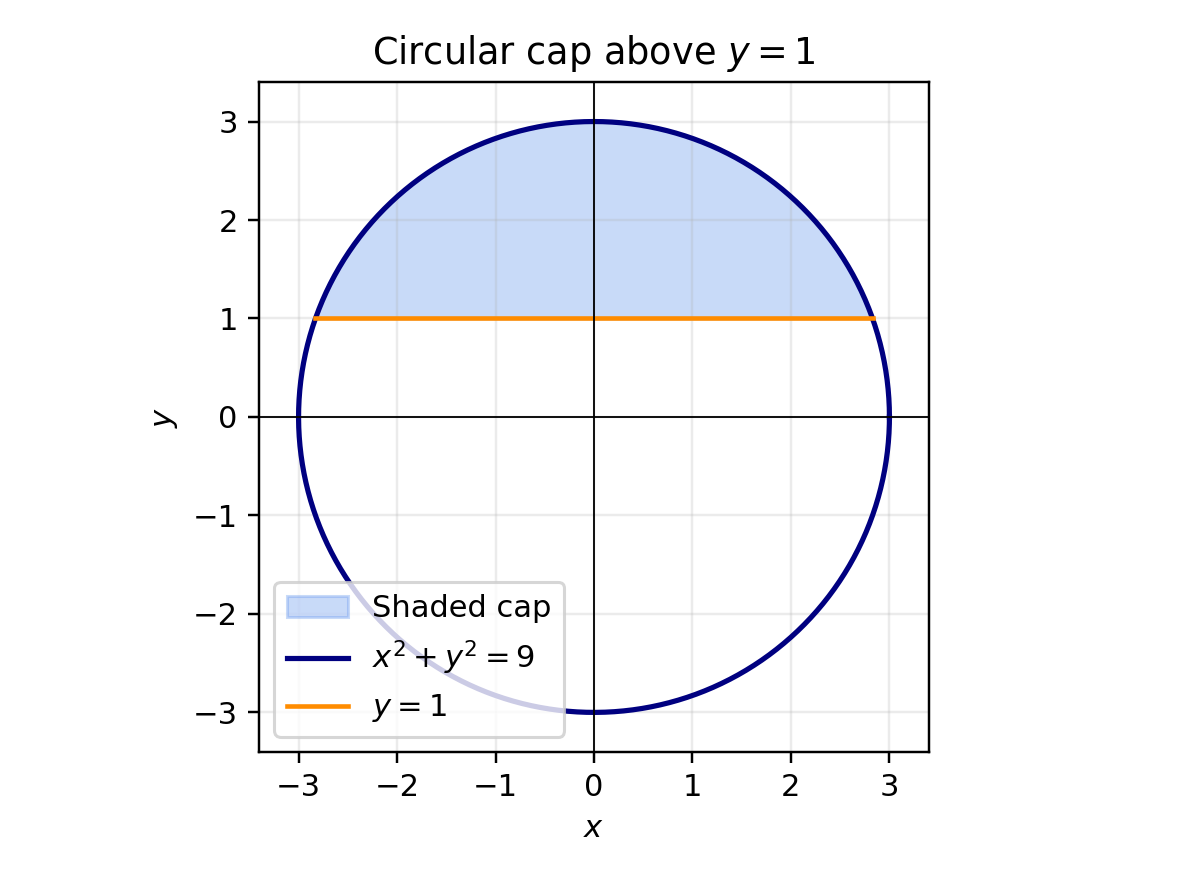
\includegraphics[width=0.48\linewidth]{figs/2.2.6.png}\caption{Circle $x^2+y^2=9$ and the cap above $y=1$.}\end{figure}

\item[2.2.7] If $(\vec a+\vec b)\cdot(\vec a-\vec b)=198$ and $|\vec a|=10|\vec b|$, select the true statement.

\begin{multicols}{2}
\begin{enumerate}
\setlength{\itemsep}{0pt}
    \item $|\vec a|=\sqrt2$
    \item $|\vec b|=\sqrt2$
    \item $|\vec b|=10\sqrt2$
    \item $|\vec a|=10/\sqrt2$\nobreak\hfill\mbox{(12,2026)}
\end{enumerate}
\end{multicols}



\vspace{0.6em}\par\solution


Using $(\vec a+\vec b)\cdot(\vec a-\vec b)=|\vec a|^2-|\vec b|^2$, let $r=|\vec b|\ge0$. Since $|\vec a|=10r$,
\[
100r^2-r^2=198,\qquad r^2=2.
\]
The reduced convex problem is
\[
\text{maximize }r\quad\text{subject to }r\ge0,\quad r^2\le2.
\]
Its largest feasible value is $r=\sqrt2$, so $|\vec b|=\sqrt2$ and the answer is \textbf{b)}. CVXPY solves this reduced scalar problem.
\par\noindent\hfill\mbox{\textit{(\ref{formula-2-1-9})}}\par\begin{lstlisting}[frame=single, basicstyle=\rmfamily, escapeinside={(*@}{@*)}]
(*@\makebox[\dimexpr\linewidth-2\fboxsep-2\fboxrule\relax][c]{codes/2.2.7.py}@*)
\end{lstlisting}

\item[2.2.8] Find the sub-interval(s) of $(0,\pi/2)$ in which $f(x)=\tan x-4x$ is increasing.\nobreak\hfill\mbox{(12,2026)}



\vspace{0.6em}\par\solution


$f'(x)=\sec^2x-4>0$ precisely when $\cos x<1/2$ on this domain, so the critical point is $x=\pi/3$. Therefore $f$ is increasing on $\boxed{(\pi/3,\pi/2)}$. The Python code uses bisection to locate the zero of $f'(x)$ numerically and plots $f$, shading the interval where it increases.
\par\noindent\hfill\mbox{\textit{(\ref{formula-2-1-3}, \ref{formula-2-1-4}, \ref{formula-2-1-18})}}\par\begin{lstlisting}[frame=single, basicstyle=\rmfamily, escapeinside={(*@}{@*)}]
(*@\makebox[\dimexpr\linewidth-2\fboxsep-2\fboxrule\relax][c]{codes/2.2.8.py}@*)
\end{lstlisting}
\begin{figure}[H]\centering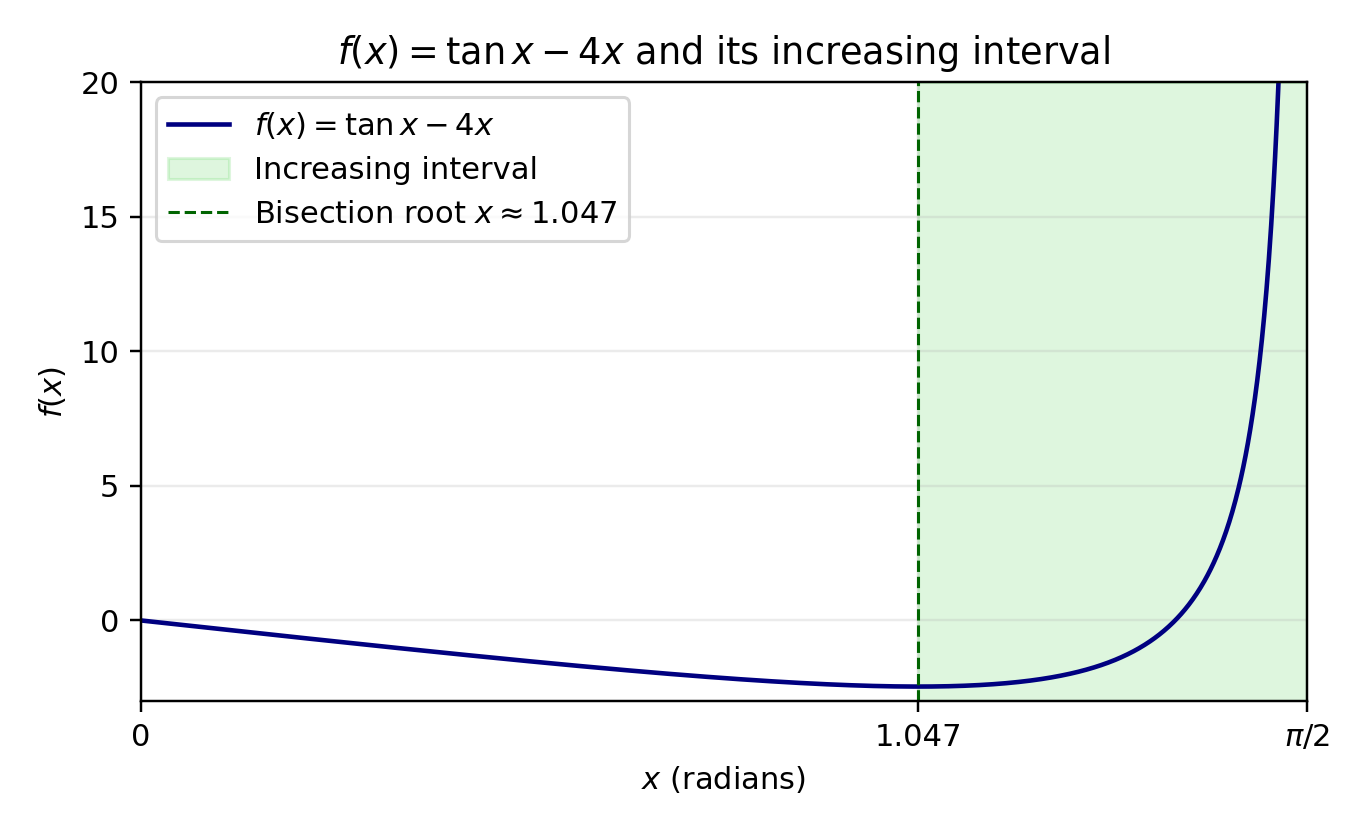
\includegraphics[width=0.68\linewidth]{figs/2.2.8.png}\caption{The function rises on the shaded interval.}\end{figure}

\item[2.2.9] For unit vectors $\vec a,\vec b$, if $|\vec a+2\vec b|=|2\vec a-\vec b|$, find the angle between them.\nobreak\hfill\mbox{(12,2026)}



\vspace{0.6em}\par\solution


Let $c=\vec a\cdot\vec b$. Since $|\vec a|=|\vec b|=1$, their Gram matrix is
\[
G=\begin{bmatrix}1&c\\c&1\end{bmatrix}.
\]
The squared lengths are
\[
|\vec a+2\vec b|^2=
\begin{bmatrix}1&2\end{bmatrix}G\begin{bmatrix}1\\2\end{bmatrix}=5+4c,
\qquad
|2\vec a-\vec b|^2=
\begin{bmatrix}2&-1\end{bmatrix}G\begin{bmatrix}2\\-1\end{bmatrix}=5-4c.
\]
The given equality implies $5+4c=5-4c$, so $c=0$. Thus $\cos\theta=\vec a\cdot\vec b=0$, and the angle is $\boxed{90^\circ}$.\par\noindent\hfill\mbox{\textit{(\ref{formula-2-1-9}, \ref{formula-2-1-19})}}\par

\item[2.2.10]
(a) If $\frac{x-3}{1}=\frac{1-y}{1}=\frac{z+2}{p}$ and $\frac{2-x}{3}=\frac{y+1}{5}=\frac{z+56}{2p}$ are perpendicular, find $p$.\\
\textbf{OR}\\
(b) Find the vector equation of the line through the origin perpendicular to both $\vec r=2\hat i-\hat j+2\hat k+\lambda(3\hat i+4\hat j+2\hat k)$ and $\vec r=\mu(\hat i-\hat j+\hat k)$.\nobreak\hfill\mbox{(12,2026)}



\vspace{0.6em}\par\solution


(a) The direction vectors are $(1,-1,p)$ and $(-3,5,2p)$. Their dot product is $2p^2-8$, so $\boxed{p=\pm2}$.\\
(b) Let the required direction be $(a,b,c)$. Perpendicularity gives $3a+4b+2c=0$ and $a-b+c=0$. Taking $b=1$ gives $a=-6$, $c=7$. Thus the line is $\boxed{\vec r=t(-6\hat i+\hat j+7\hat k)}$. The Python code verifies both dot products and plots the vectors without using a cross product.
\par\noindent\hfill\mbox{\textit{(\ref{formula-2-1-9}, \ref{formula-2-1-11})}}\par\begin{lstlisting}[frame=single, basicstyle=\rmfamily, escapeinside={(*@}{@*)}]
(*@\makebox[\dimexpr\linewidth-2\fboxsep-2\fboxrule\relax][c]{codes/2.2.10.py}@*)
\end{lstlisting}
\begin{figure}[H]\centering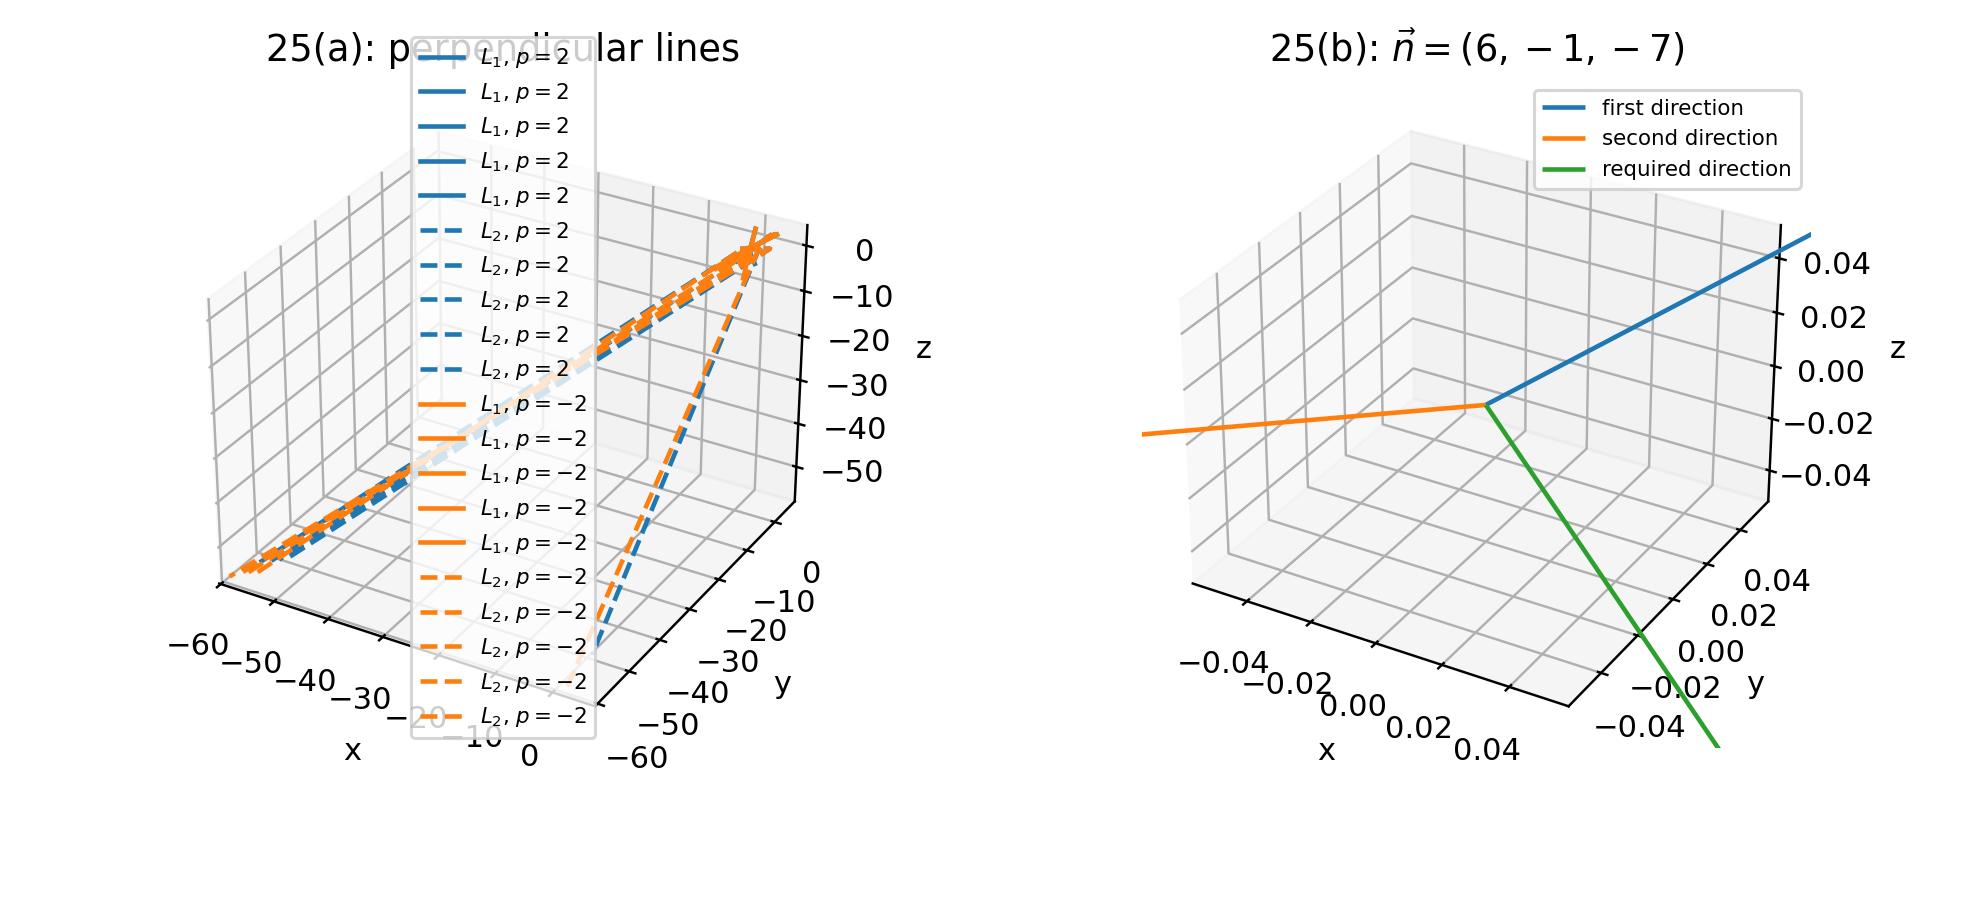
\includegraphics[width=0.75\linewidth]{figs/2.2.10.png}\caption{Direction diagrams for the two alternatives in Question 25.}\end{figure}

\item[2.2.11] Robotic knee replacement surgery has a $90\%$ success rate. For three independent surgeries, find the probability that (i) exactly one succeeds, and (ii) at most two succeed.\nobreak\hfill\mbox{(12,2026)}



\vspace{0.6em}\par\solution


Let $X$ be the number of successful surgeries. Independence gives the PMF
\[
p_X(k)=\binom{3}{k}(0.9)^k(0.1)^{3-k},\qquad k=0,1,2,3.
\]
Its values are
\[
\begin{array}{c|cccc}
k&0&1&2&3\\\hline
p_X(k)&0.001&0.027&0.243&0.729
\end{array}.
\]
(i) $P(X=1)=p_X(1)=\boxed{0.027}$. (ii) $P(X\le2)=p_X(0)+p_X(1)+p_X(2)=0.001+0.027+0.243=\boxed{0.271}$.\par\noindent\hfill\mbox{\textit{(\ref{formula-2-1-8}, \ref{formula-2-1-20})}}\par

\item[2.2.12] Show that $f:\mathbb R\to\mathbb R$, $f(x)=\frac{x}{\sqrt{1+x^2}}$, is one-one but not onto.\nobreak\hfill\mbox{(12,2026)}



\vspace{0.6em}\par\solution

$f'(x)=(1+x^2)^{-3/2}>0$, so $f$ is strictly increasing and therefore one-one. Also $|f(x)|<1$ for every real $x$, and its range is $(-1,1)$, so it is not onto $\mathbb R$. The plot illustrates the range.
\par\noindent\hfill\mbox{\textit{(\ref{formula-2-1-3}, \ref{formula-2-1-18})}}\par
\begin{lstlisting}[frame=single, basicstyle=\rmfamily, escapeinside={(*@}{@*)}]
(*@\makebox[\dimexpr\linewidth-2\fboxsep-2\fboxrule\relax][c]{codes/2.2.12.py}@*)
\end{lstlisting}
\begin{figure}[H]\centering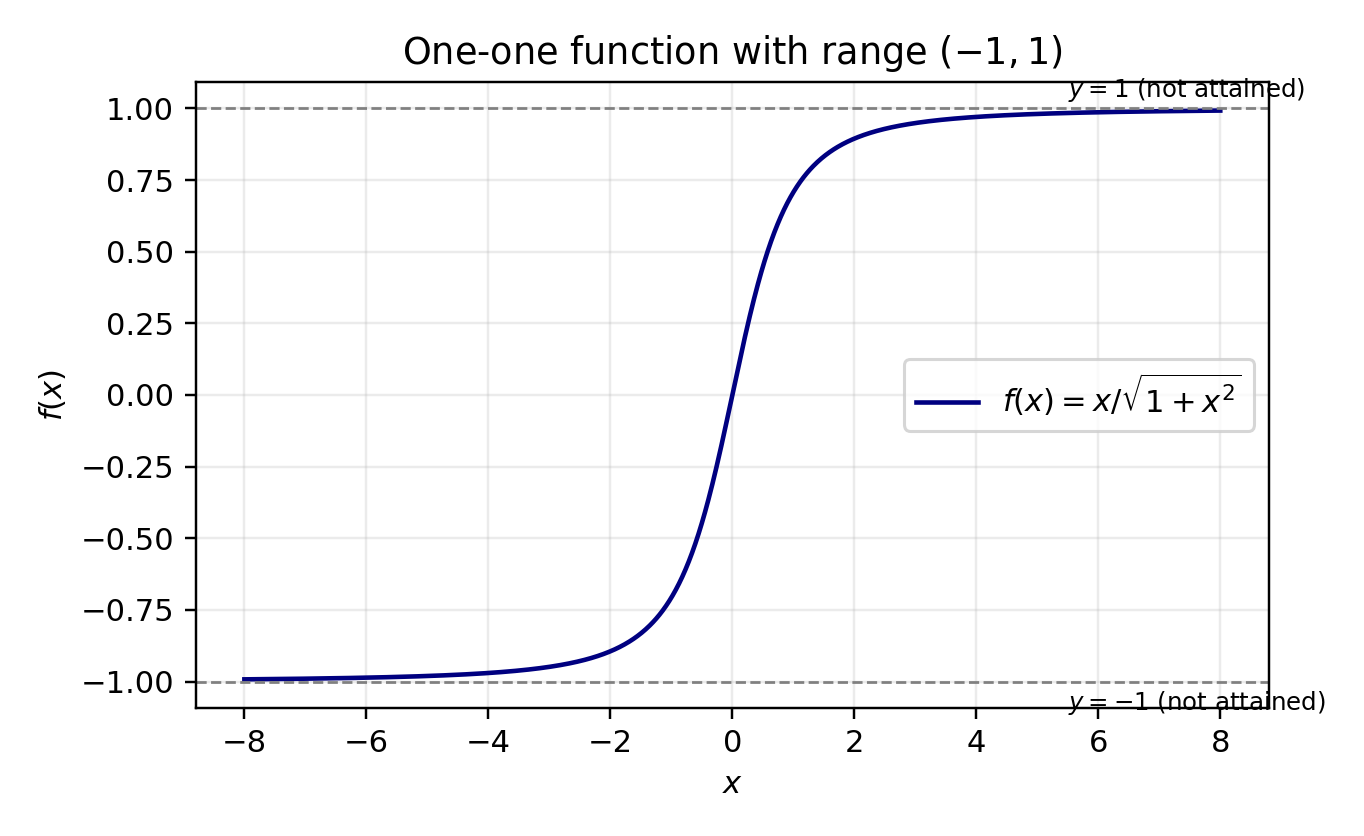
\includegraphics[width=0.68\linewidth]{figs/2.2.12.png}\caption{The function is strictly increasing and approaches, but never reaches, $\pm1$.}\end{figure}

\item[2.2.13] Solve graphically: maximize $Z=600x+400y$ subject to $x+2y\le12$, $4x+5y\ge20$, $2x+y\le12$, and $x,y\ge0$.\nobreak\hfill\mbox{(12,2026)}



\vspace{0.6em}\par\solution


The feasible vertices are $(0,4),(0,6),(4,4),(6,0),(5,0)$. Evaluating $Z$ gives $1600,2400,4000,3600,3000$, respectively. Thus $\boxed{Z_{\max}=4000}$ at $(4,4)$. The Python code uses CVXPY to solve the linear program and uses CoordGeo to plot the constraints and label the feasible vertices.
\par\noindent\hfill\mbox{\textit{(\ref{formula-2-1-10})}}\par\begin{lstlisting}[frame=single, basicstyle=\rmfamily, escapeinside={(*@}{@*)}]
(*@\makebox[\dimexpr\linewidth-2\fboxsep-2\fboxrule\relax][c]{codes/2.2.13.py}@*)
\end{lstlisting}
\begin{figure}[H]\centering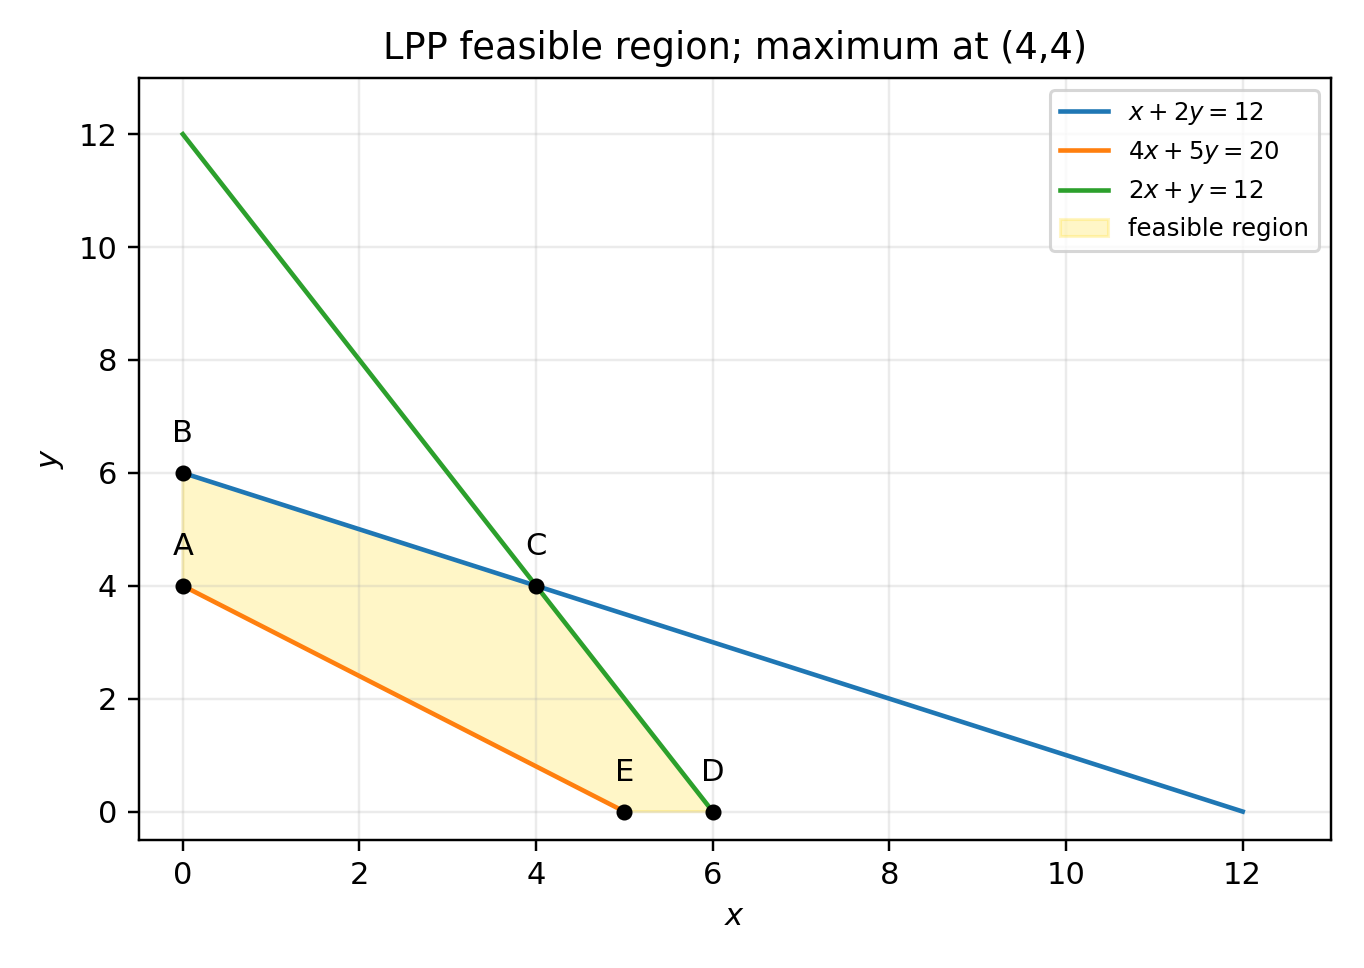
\includegraphics[width=0.68\linewidth]{figs/2.2.13.png}\caption{The shaded feasible region has its maximum at $(4,4)$.}\end{figure}

\item[2.2.14]
\noindent(a) A showroom gives 60 vouchers of Rs. 1,000 and Rs. 500. The number of Rs. 1,000 vouchers plus three times the number of Rs. 500 vouchers is 100. Form the equations and find the counts by the matrix method.\\
\textbf{OR}\\
\noindent(b) Given $P=\begin{bmatrix}2&-1\\3&4\end{bmatrix}$, $Q=\begin{bmatrix}5&2\\7&4\end{bmatrix}$ and $R=\begin{bmatrix}2&5\\3&8\end{bmatrix}$, find $S$ such that $PQ-RS=O$.\nobreak\hfill\mbox{(12,2026)}



\vspace{0.6em}\par\solution


\noindent(a) Let $x,y$ denote the two voucher counts. Then $x+y=60$, $x+3y=100$. Subtracting the first equation from the second gives $2y=40$, so $y=20$ and $x=40$. Thus there are $\boxed{40}$ Rs. 1,000 vouchers and $\boxed{20}$ Rs. 500 vouchers. The Python code solves the augmented system by Gaussian elimination.\par\noindent\hfill\mbox{\textit{(\ref{formula-2-1-21})}}\\
\noindent(b) First compute $PQ=\begin{bmatrix}3&0\\43&22\end{bmatrix}$ and solve $RS=PQ$ by Gaussian elimination. This gives
\begin{equation*}
\boxed{S=\begin{bmatrix}-191&-110\\77&44\end{bmatrix}}.
\tag*{(\ref{formula-2-1-1}, \ref{formula-2-1-21})}\end{equation*}
\begin{lstlisting}[frame=single, basicstyle=\rmfamily, escapeinside={(*@}{@*)}]
(*@\makebox[\dimexpr\linewidth-2\fboxsep-2\fboxrule\relax][c]{codes/2.2.14a.py}@*)
\end{lstlisting}
\begin{lstlisting}[frame=single, basicstyle=\rmfamily, escapeinside={(*@}{@*)}]
(*@\makebox[\dimexpr\linewidth-2\fboxsep-2\fboxrule\relax][c]{codes/2.2.14b.py}@*)
\end{lstlisting}

\item[2.2.15]
(a) Write the lines $\frac{x+3}{-3}=\frac{y-1}{1}=\frac{z-5}{5}$ and $\frac{x+1}{-1}=\frac{2-y}{-2}=\frac{z-5}{5}$ in vector form and check whether they intersect.\\
\textbf{OR}\\
(b) A square has opposite sides along $\vec r=(1,2,-4)+\lambda(2,3,6)$ and $\vec r=(3,3,-5)+\mu(2,3,6)$. If the other pair has direction ratios $(-3,6,p)$, find the square's area and $p$.\nobreak\hfill\mbox{(12,2026)}



\vspace{0.6em}\par\solution


(a) The vector forms are $\vec r=(-3,1,5)+\lambda(-3,1,5)$ and $\vec r=(-1,2,5)+\mu(-1,2,5)$. At $\lambda=\mu=-1$, both pass through $(0,0,0)$, so they intersect there.\\
(b) The separation of the parallel lines is $\sqrt{293}/7$, so the square's area is $\boxed{293/49}$. Perpendicular adjacent side directions require $(2,3,6)\cdot(-3,6,p)=0$, giving $\boxed{p=-2}$. The Python code computes the line intersection, square side length, area, and $p$, then plots both configurations using CoordGeo.
\par\noindent\hfill\mbox{\textit{(\ref{formula-2-1-9}, \ref{formula-2-1-11})}}\par\begin{lstlisting}[frame=single, basicstyle=\rmfamily, escapeinside={(*@}{@*)}]
(*@\makebox[\dimexpr\linewidth-2\fboxsep-2\fboxrule\relax][c]{codes/2.2.15.py}@*)
\end{lstlisting}
\begin{figure}[H]\centering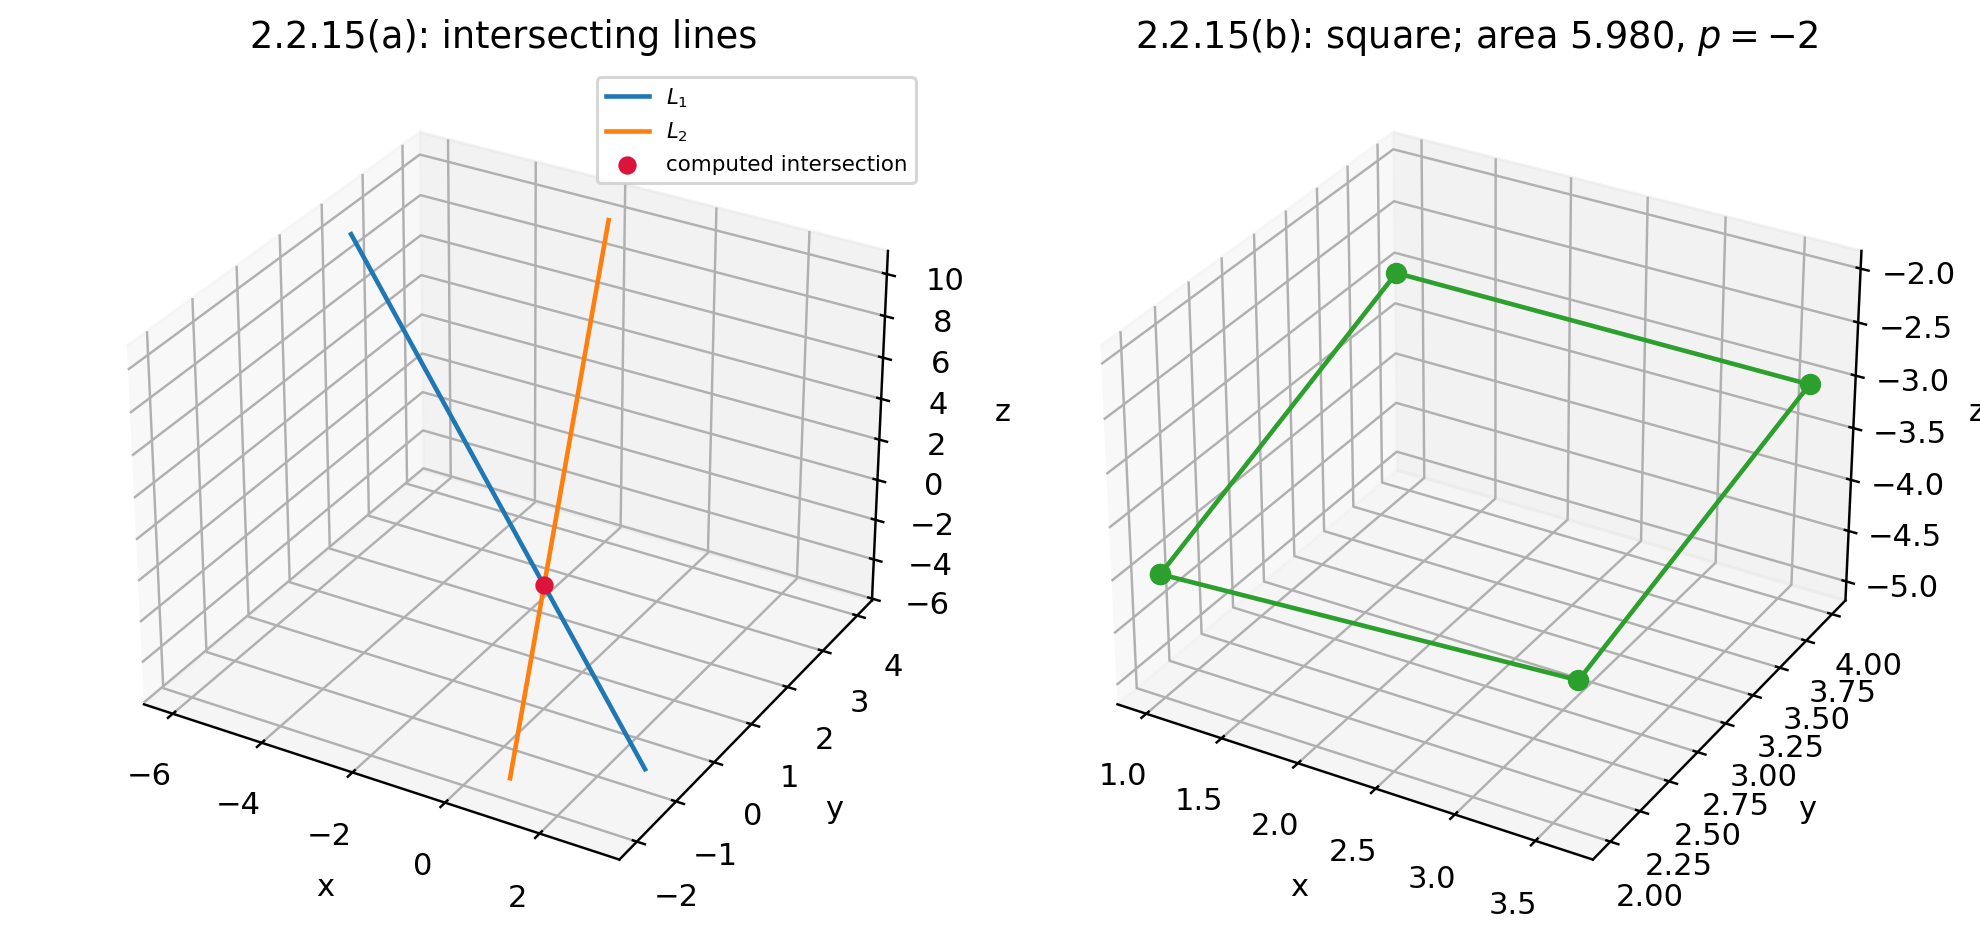
\includegraphics[width=0.75\linewidth]{figs/2.2.15.png}\caption{The two line configurations and the square between parallel lines.}\end{figure}

\item[2.2.16] Two vertical poles of heights $22$ m and $16$ m stand on opposite sides of a $20$ m road. Ladders from a point $R$, $x$ m from the shorter pole, reach their tops. (i) Express $p(x)=l_1+l_2$. (ii) Find $p'(x)$. (iii)(a) Find $x$ minimizing $l_1^2+l_2^2$. \textbf{OR} (b) if both poles are $16$ m tall, find the position minimizing the sum of squared ladder lengths.\nobreak\hfill\mbox{(12,2026)}



\vspace{0.6em}\par\solution


The horizontal distances from $R$ to the $22$ m and $16$ m poles are $20-x$ and $x$, respectively. Hence
\begin{equation*}
\begin{aligned}
l_1(x)&=\sqrt{484+(20-x)^2}, & l_2(x)&=\sqrt{256+x^2},\\
p(x)&=l_1+l_2=\sqrt{484+(20-x)^2}+\sqrt{256+x^2},\\
p'(x)&=-\frac{20-x}{\sqrt{484+(20-x)^2}}+\frac{x}{\sqrt{256+x^2}}.
\end{aligned}
\tag*{(\ref{formula-2-1-3}, \ref{formula-2-1-4})}\end{equation*}
For (a),
\[
l_1^2+l_2^2=484+(20-x)^2+256+x^2=2(x-10)^2+940,
\]
so the minimum occurs at $\boxed{x=10\text{ m}}$.
For (b), if both poles are $16$ m tall, the sum of squared ladder lengths is
\[
[256+(20-x)^2]+[256+x^2]=2(x-10)^2+712,
\]
which is minimized when $\boxed{x=10\text{ m}}$, the midpoint of the road. The CVXPY code independently minimizes the squared-length objective for both height configurations and prints the optimal position and minimum value.
\par\begin{lstlisting}[frame=single, basicstyle=\rmfamily, escapeinside={(*@}{@*)}]
(*@\makebox[\dimexpr\linewidth-2\fboxsep-2\fboxrule\relax][c]{codes/2.2.16.py}@*)
\end{lstlisting}

\item[2.2.17] Of students taking an entrance examination, $40\%$ are dropouts and $60\%$ are regular students. The pass rates are $5\%$ for dropouts and $10\%$ for regular students. Find (i) the probability a student is regular, (ii) the probability a dropout fails, (iii)(a) given a student passed, the probability they are not a dropout, \textbf{OR} (b) given a student failed, the probability they were regular.\nobreak\hfill\mbox{(12,2026)}



\vspace{0.6em}\par\solution


Let $X$ denote the student's type ($D$: dropout, $R$: regular), and $Y$ the result ($S$: pass, $F$: fail). Their joint PMF is
\[
p_{X,Y}(x,y)=P(X=x)P(Y=y\mid X=x),
\]
The joint PMF and its marginals are
\[
\begin{array}{c|cc|c}
X\backslash Y & S & F & p_X(x)\\\hline
D & 0.02 & 0.38 & 0.40\\
R & 0.06 & 0.54 & 0.60\\\hline
p_Y(y) & 0.08 & 0.92 & 1
\end{array}.
\]
Using the joint PMF and its marginals,
\begin{align*}
\text{(i)}\quad&P(X=R)=0.06+0.54=\boxed{0.60}.\\
\text{(ii)}\quad&P(Y=F\mid X=D)=\frac{0.38}{0.40}=\boxed{0.95}.\\[2pt]
\text{(iii)(a)}\quad&P(X=R\mid Y=S)=\frac{0.06}{0.08}=\boxed{\frac34}.\\[2pt]
\text{(iii)(b)}\quad&P(X=R\mid Y=F)=\frac{0.54}{0.92}=\boxed{\frac{27}{46}}.
\tag*{(\ref{formula-2-1-8}, \ref{formula-2-1-12}, \ref{formula-2-1-20})}\end{align*}

\item[2.2.18] A triangular park has vertices $A(0,4)$, $B(-2,0)$ and $C(3,0)$, with $O=(0,0)$. Find (i) the equation of $AB$, (ii) the equation of $AC$, and (iii)(a) the area of $OAC$ by integration, \textbf{OR} (b) the area of $AOB$ by integration.\nobreak\hfill\mbox{(12,2026)}



\vspace{0.6em}\par\solution


Using the slopes from the given vertices,
\[
AB:\ y=2x+4,\qquad AC:\ y=4-\frac43x.
\]
For (a), split $[0,3]$ into $n$ equal steps of width $h=3/n$, with $x_k=kh$. Let $A_0=0$ and accumulate each rectangle by the difference equation
\[
A_{k+1}-A_k=h\left(4-\frac43x_k\right).
\]
Summing the recurrence gives
\[
\begin{aligned}
A_n&=\frac3n\sum_{k=0}^{n-1}\left(4-\frac{4k}{n}\right)=6+\frac6n\longrightarrow 6,\\
\therefore\quad \operatorname{area}(OAC)&=\boxed{6\text{ square units}}.
\end{aligned}
\]
\newpage
For (b), take $h=2/n$, $x_k=-2+2k/n$, and $B_0=0$. The corresponding recurrence and sum are
\[
B_{k+1}-B_k=h(2x_k+4),\qquad
B_n=\frac2n\sum_{k=0}^{n-1}\frac{4k}{n}=4\left(1-\frac1n\right)\longrightarrow4,
\]
so $\operatorname{area}(AOB)=\boxed{4\text{ square units}}$. These accumulated rectangle sums converge to the definite integrals in the question. The plot code uses CoordGeo's line generator and point-labeling function.
\par\noindent\hfill\mbox{\textit{(\ref{formula-2-1-5}, \ref{formula-2-1-17})}}\par
\begin{lstlisting}[frame=single, basicstyle=\rmfamily, escapeinside={(*@}{@*)}]
(*@\makebox[\dimexpr\linewidth-2\fboxsep-2\fboxrule\relax][c]{codes/2.2.18.py}@*)
\end{lstlisting}
\begin{figure}[H]\centering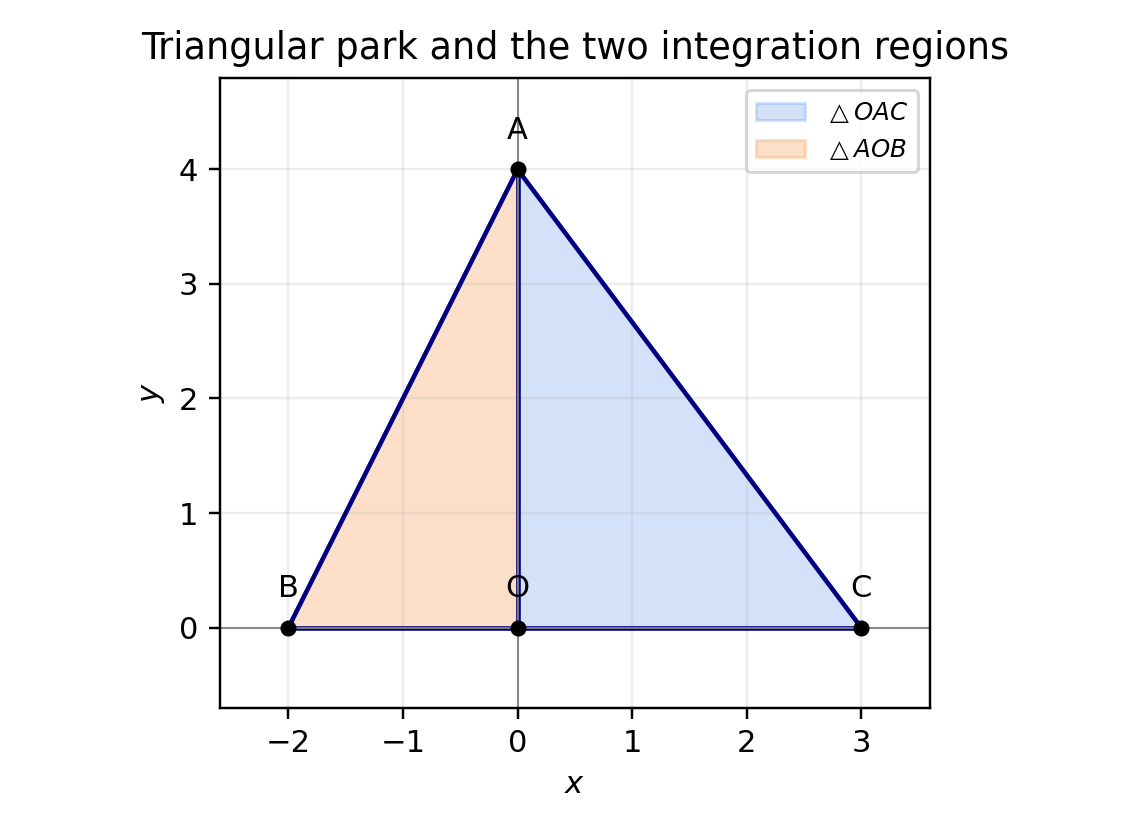
\includegraphics[width=0.55\linewidth]{figs/2.2.18.png}\caption{The shaded regions $OAC$ and $AOB$ are evaluated by integration.}\end{figure}
\end{enumerate}


\end{document}
